%%%%%%%%%%%%%
%% METHODS %%
%%%%%%%%%%%%%

%This chapter describes in detail the methods for whatever activities were necessary for your project – e.g., data gathering, data analysis, requirements analysis, design, implementation, testing/evaluation, etc. Your choice of methods should be discussed and justified in view of the project objectives, and with reference to the pertinent literature. Report not only what methods you applied in generic terms, but what you actually did: sufficient information about dates and details for your reader to understand how you ran your project, rather than just how one could run any similar project. 

\chapter{Methods}
\label{Methods} 

\section*{List of Abbreviations}
\label{sec:abbreviations}
\addcontentsline{toc}{section}{List of Abbreviations}

\begin{description}
    \item[CNN] Convolutional Neural Network
    \item[GPU] Graphics Processing Unit
    \item[HPC] High-Performance Computing
    \item[QLoRA] Quantized Low-Rank Adaptation
    \item[ViT] Vision Transformer
    \item[VLM] Vision-Language Model
\end{description}

\section{Simulators}

In this section we examine some simulators currently available to the task of training autonomous systems, to the be able to consider safety aspects of such models.

\subsection{AirSim}

The AirSim \cite{airsim2017fsr} is a simulator for autonomous vehicles, aimed to be a platform for AI research.

The paper was accepted for the Field and Service Robotics 10th International Conference. No other papers seam to deal with simulators, at least in the title. AirSim references 23 articles.

\subsection{Applying Noise to Images}

\subsection{Carla}

\subsection{weight initialisation}

\subsection{MNIST Dataset}

The MNIST dataset, a cornerstone in the field of machine learning, serves as a benchmark for evaluating the performance of algorithms in the domain of handwritten digit recognition. Comprising a collection of 70,000 grayscale images, each of 28x28 pixel resolution, the dataset is divided into two distinct sets: a training set containing 60,000 examples, and a test set with 10,000 examples (\cite{LeCun1998}). Each image within the dataset is associated with a label from 0 to 9, corresponding to the digit it represents.

This dataset has been instrumental in facilitating advancements in machine learning, particularly in the development and evaluation of algorithms capable of performing classification tasks. Its widespread adoption can be attributed to several factors, including the simplicity of the task it presents and its suitability for use in benchmarking the performance of various learning algorithms, ranging from simple linear classifiers to more complex deep learning models.

A key feature of the MNIST dataset is its pre-processing stage, where the digits have been size-normalized and centered in a fixed-size image. This pre-processing reduces the variability unrelated to digit identity, allowing researchers to focus on the algorithmic challenge of digit recognition rather than on the preprocessing steps.

The significance of the MNIST dataset in the realm of machine learning research is well-documented, with \cite{LeCun1998} providing an extensive overview of the dataset's creation, characteristics, and its role in fostering advancements in the field.

This foundational dataset has not only enabled the comparison of algorithmic performance in a standardized setting but has also contributed to the proliferation of research in neural networks, serving as a pivotal benchmark for innovations in the field.

% Dataset description

The MNIST dataset is comprised of two main components: image files and label files, structured as follows:

\begin{itemize}
    \item \textbf{Training Set Images:} Contains 60,000 training examples.
    \item \textbf{Test Set Images:} Contains 10,000 test examples.
    \item Each image is encoded as a 28x28 pixel grid, summing up to 784 pixels per image. Each pixel represents a grayscale intensity, with 0 and 255 denote black and white respectively.
\end{itemize}

The structure of the image files is detailed below:
\begin{enumerate}
    \item \textbf{Magic Number:} The first 4 bytes signify a magic number (2051) that identifies the file format.
    \item \textbf{Number of Images:} The following 4 bytes denote the count of images, encoded as a 32-bit integer.
    \item \textbf{Rows:} The subsequent 4 bytes illustrate the number of rows (28) per image, encoded as a 32-bit integer.
    \item \textbf{Columns:} The next 4 bytes depict the number of columns (28) per image, encoded as a 32-bit integer.
    \item \textbf{Pixel Values:} The remainder of the file is populated with pixel values in row-major order, with each image delineated sequentially in the file. Each pixel value is stored as an unsigned byte, representing the pixel's intensity.
\end{enumerate}

and label files:
\begin{itemize}
    \item \textbf{Training Set Labels:} Comprises 60,000 labels corresponding to the training images.
    \item \textbf{Test Set Labels:} Comprises 10,000 labels corresponding to the test images.
    \item Each label is a single byte signifying the digit (0 through 9) that the corresponding image represents.
\end{itemize}

The structure of the label files is detailed below:
\begin{enumerate}
    \item \textbf{Magic Number:} The first 4 bytes signify a magic number (2049) that identifies the file format.
    \item \textbf{Number of Items:} The following 4 bytes denote the count of labels, encoded as a 32-bit integer.
    \item \textbf{Labels:} The remainder of the file contains label values, stored as unsigned bytes, with each label corresponding to the image of the same index in the image file.
\end{enumerate}

This standardized format ensures the MNIST dataset's compatibility with a wide array of machine learning models, particularly facilitating research in image classification and handwriting recognition.

\begin{table}[h]
\centering
\begin{tabular}{|l|l|r|r|}
\hline
\textbf{Type}             & \textbf{File Name}                       & \textbf{Size (B)} & \textbf{Count} \\ \hline
Training Images & \texttt{train-images-idx3-ubyte} & 47040016           & 60000 \\
Training Labels & \texttt{train-labels-idx1-ubyte} & 60008             & 60000 \\
Testing Images  & \texttt{t10k-images-idx3-ubyte}  & 7840016           & 10000 \\
Testing Labels  & \texttt{t10k-labels-idx1-ubyte}  & 10008              & 10000 \\ \hline
\end{tabular}
\caption{MNIST Dataset Files, file sizes in bytes and image/label count}
\label{table:mnist_files_b}
\end{table}
The contents can be examined with the \textit{xxd} command:
\begin{verbatim}
!xxd -C 'data/MNIST/raw/train-images-idx3-ubyte' | head

00000000: 0000 0803 0000 ea60 0000 001c 0000 001c  .......`........
00000010: 0000 0000 0000 0000 0000 0000 0000 0000  ................
00000020: 0000 0000 0000 0000 0000 0000 0000 0000  ................
00000030: 0000 0000 0000 0000 0000 0000 0000 0000  ................
00000040: 0000 0000 0000 0000 0000 0000 0000 0000  ................
00000050: 0000 0000 0000 0000 0000 0000 0000 0000  ................
00000060: 0000 0000 0000 0000 0000 0000 0000 0000  ................
00000070: 0000 0000 0000 0000 0000 0000 0000 0000  ................
00000080: 0000 0000 0000 0000 0000 0000 0000 0000  ................
00000090: 0000 0000 0000 0000 0000 0000 0000 0000  ................

!xxd -C 'data/MNIST/raw/train-labels-idx1-ubyte' | head

00000000: 0000 0801 0000 ea60 0500 0401 0902 0103  .......`........
00000010: 0104 0305 0306 0107 0208 0609 0400 0901  ................
00000020: 0102 0403 0207 0308 0609 0005 0600 0706  ................
00000030: 0108 0709 0309 0805 0903 0300 0704 0908  ................
00000040: 0009 0401 0404 0600 0405 0601 0000 0107  ................
00000050: 0106 0300 0201 0107 0900 0206 0708 0309  ................
00000060: 0004 0607 0406 0800 0708 0301 0507 0107  ................
00000070: 0101 0603 0002 0903 0101 0004 0902 0000  ................
00000080: 0200 0207 0108 0604 0106 0304 0509 0103  ................
00000090: 0308 0504 0707 0402 0805 0806 0703 0406  ................
\end{verbatim}

% Sanity check - number of files ~ 7260000 
% hex(7260000)
% '0x6ec760'
% int('006ec760', 16)
% 7260000 ~ pmnist training dataset
% int('001339e0', 16)
% 1260000 ~ pmnist testing dataset

% xxd perturbed-train-images-idx3-ubyte
% 00000000: 0000 0803 006e c760 0000 001c 0000 001c  .....n.`........
% xxd perturbed-train-labels-idx1-ubyte
% 00000000: 0000 0801 006e c760                      .....n.`
% xxd perturbation-train-levels-idx0-ubyte
% 00000000: 0000 07ff 006e c760                      .....n.`
% xxd t1260k-perturbed-images-idx3-ubyte
% 00000000: 0000 0803 0013 39e0 0000 001c 0000 001c  ......9.........
% xxd t1260k-perturbed-labels-idx1-ubyte
% 00000000: 0000 0801 0013 39e0                      ......9.
% xxd t1260k-perturbation-levels-idx0-ubyte
% 00000000: 0000 07ff 0013 39e0                      ......9.


Where hex \textbf{0000 0803} is the magic number 2051 (images), and hex \textbf{0000 0801} is the magic number 2049 (labels), hex \textbf{0000 ea60}, 60,000 decimal, is the number of examples in the dataset, and hex \textbf{0000 001c}, decimal 28, is the number of rows, and columns, in every image. Therefore the number of bytes in train-images-idx3-ubyte is $4 * 4 + 60000 * 28 * 28 = 47,040,016$.

The first image in the training dataset can be obtained by offsetting the first 16 bytes (magic number, number of images, row size and column size) and taking the next 784 bytes, then splitting the array into 28 rows.


\begin{figure}[h]
    \centering
    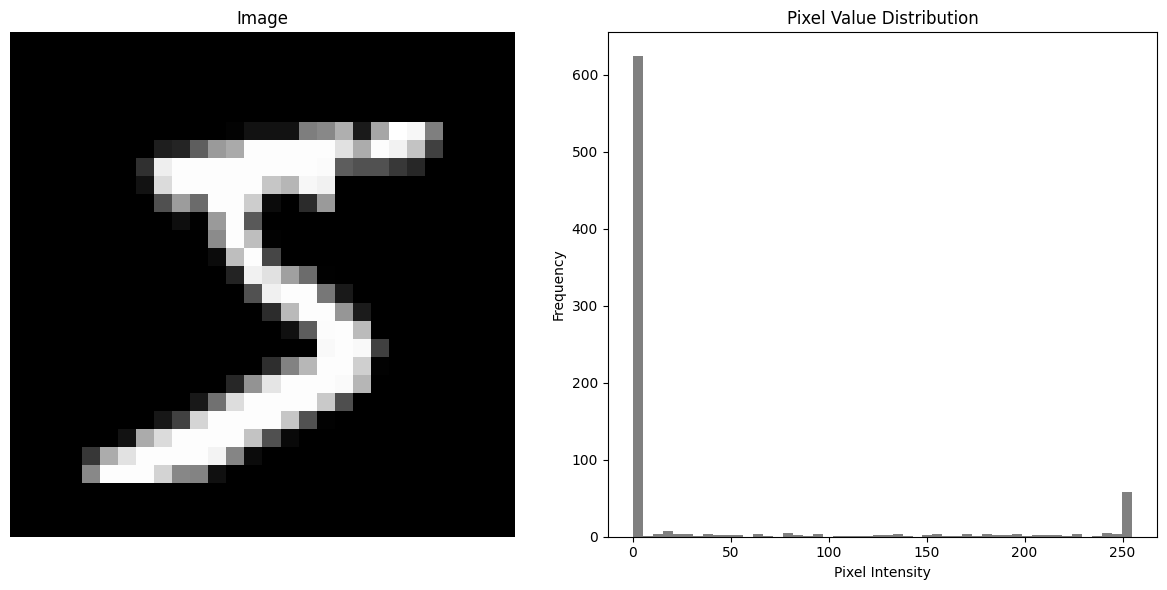
\includegraphics[width=0.75\textwidth]{Figures/Methods/MNIST_5_with_histogram.png}
    \caption{MNIST digit 5 and its pixel value distribution histogram.}
    \label{fig:mnist_5_histogram}
\end{figure}
As shown in Figure~\ref{fig:mnist_5_histogram}, the MNIST digit 5 is displayed alongside its pixel value distribution histogram where the pixel values range from 0 to 255. Figure~\ref{fig:mnist_0_histogram} shows the second image (zero) in the MNIST training dataset.

\begin{figure}[h]
    \centering
    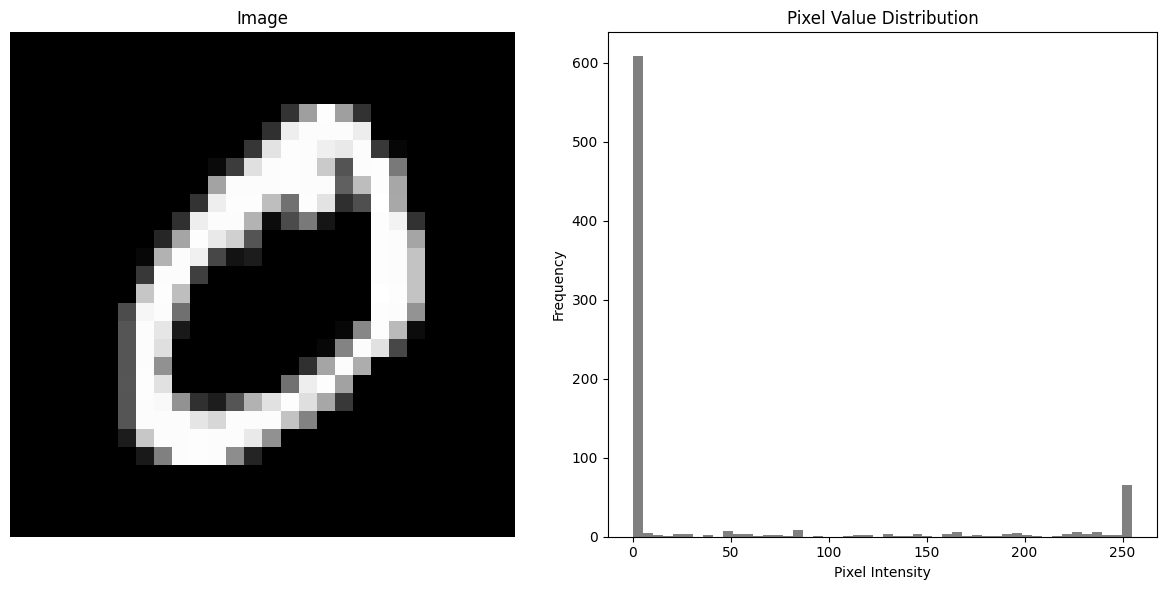
\includegraphics[width=0.75\textwidth]{Figures/Methods/MNIST_0_with_histogram.png}
    \caption{MNIST digit 0 and its pixel value distribution histogram.}
    \label{fig:mnist_0_histogram}
\end{figure}

From the training labels dataset, it can be seen that by offsetting the magic number and the number of labels, represented by 4 bytes each, the following bytes represent the labels, that is, the first two labels are "05 and "00", matching figures \ref{fig:mnist_5_histogram} and \ref{fig:mnist_0_histogram}.

\subsection{Creating the "noisy" MNIST dataset}

To augment the research on image recognition robustness, we propose the creation of an enhanced training and testing dataset derived from the original MNIST dataset. This new dataset will incorporate a variety of perturbations to the original images, aiming to simulate real-world conditions where image data may not be ideal. Specifically, we will introduce noise to the images using 12 distinct functions designed to add perturbations, categorized as follows:

\begin{enumerate}
    \item \textbf{Pixel Intensity Adjustment:}
    \begin{itemize}
        \item Brightness
        \item Contrast
    \end{itemize}
    \item \textbf{Blurring:}
    \begin{itemize}
        \item Defocus Blur
        \item Motion Blur
        \item Zoom Blur
    \end{itemize}
    \item \textbf{Noise:}
    \begin{itemize}
        \item Gaussian Noise
        \item Impulse Noise
        \item Shot Noise
    \end{itemize}
    \item \textbf{Weather:}
    \begin{itemize}
        \item Fog
        \item Frost
        \item Snow
    \end{itemize}
    \item \textbf{Special Effects:}
    \begin{itemize}
        \item Pixelation
    \end{itemize}
\end{enumerate}

Each image in the original testing dataset will undergo transformation by all perturbation methods, resulting in a companion image that retains the original label but exhibits the added noise or effect. The new dataset will consist of of the clean (original) and the noisy (perturbed) versions. 
**TODO, describe new method storing perturbation and level in lower and upper nibbles.**
To distinguish and subsequent analysis, labels will be appended to denote the image type: "0xFF" for clean/original images and "01" for noisy/perturbed images. This dual dataset structure will enable comprehensive evaluation of machine learning models' performance in recognizing digits under varied conditions, thereby enhancing the robustness of our image recognition pipeline.

% Applying noise

To generate our new dataset, we write to a binary file named perturbed-train-images-idx3-ubyte, where the first 16 bytes are:
\begin{verbatim}
0000 0803 0001 d4c0 0000 001c 0000 001c    
\end{verbatim}
Where 0001 d4c0 hex is 120000 decimal, the size of the new training dataset, twice the size of the original dataset.

We make a random selection of a perturbation type, and a perturbation level ranging from 0 to 9, and apply the perturbation to the image.

Figures \ref{fig:MNIST_4_clean_with_histogram} and \ref{fig:MNIST_4_noisy_with_histogram} show digit 4 with no noise and zoom blur level 8 applied.
\begin{figure}[h]
    \centering
    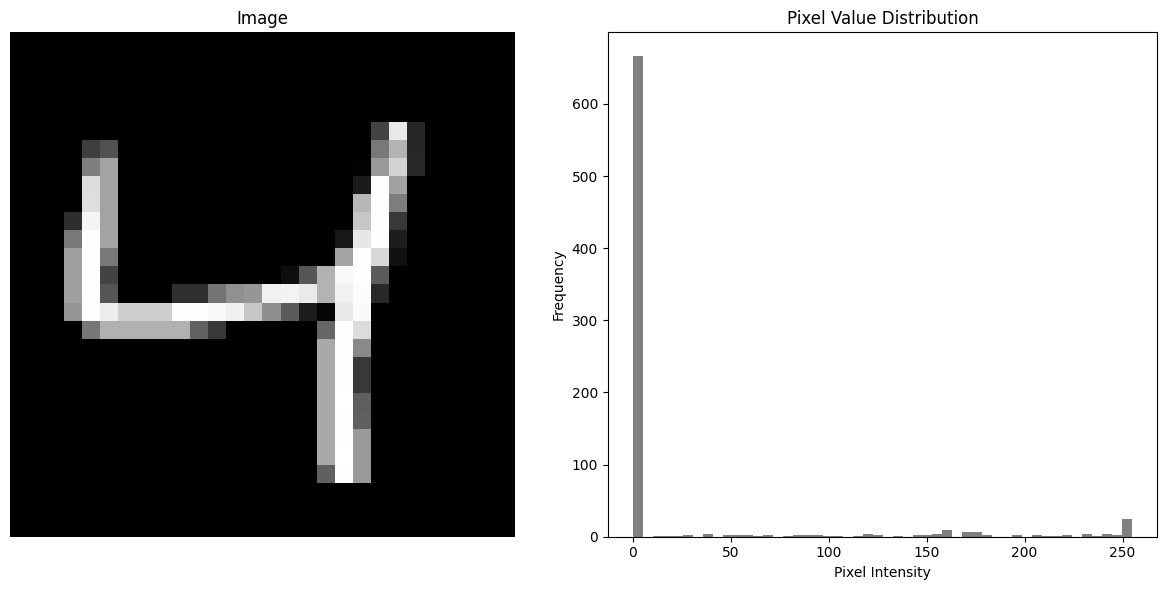
\includegraphics[width=0.75\textwidth]{Figures/Methods/MNIST_4_clean_with_histogram.png}
    \caption{MNIST digit 4 with no noise.}
    \label{fig:MNIST_4_clean_with_histogram}
\end{figure}

\begin{figure}[h]
    \centering
    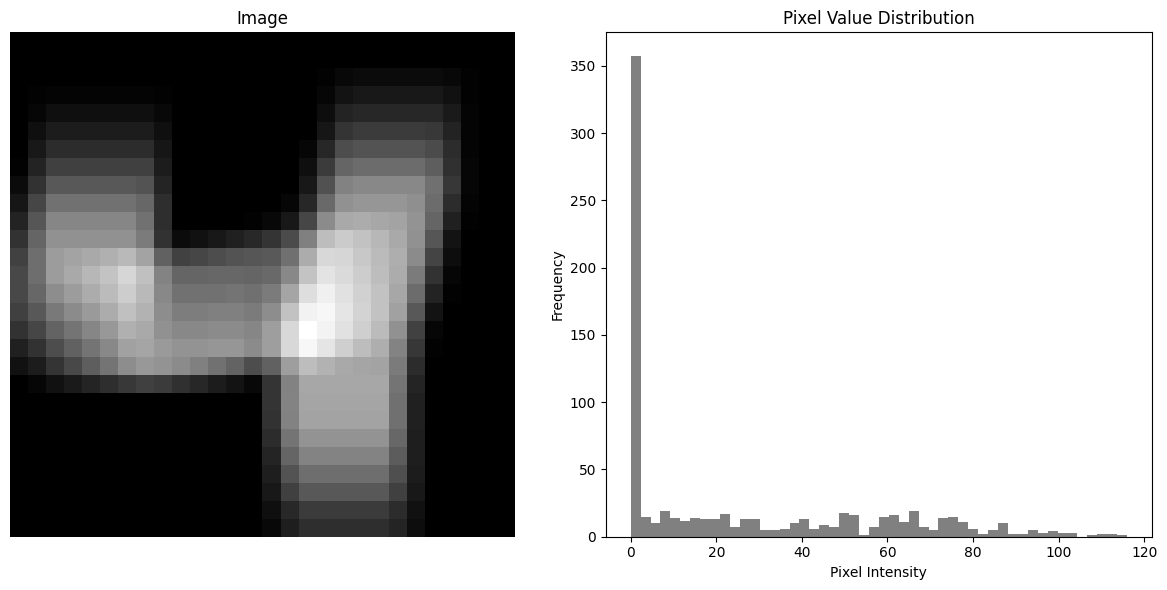
\includegraphics[width=0.75\textwidth]{Figures/Methods/MNIST_4_noisy_with_histogram.png}
    \caption{MNIST digit 4 with Zoom Blur level 8.}
    \label{fig:MNIST_4_noisy_with_histogram}
\end{figure}

% file to generate images is
% https://colab.research.google.com/drive/1s-KBSwUtT7tp280iLi8KgyHk4zThDnKD#scrollTo=OMq-a-wuKqR0
% MNIST-Dataset.ipynb

The process can be describe like so:

\begin{lstlisting}[caption={MNIST Perturbation Algorithm}, label={lst:mnist_perturbation_algorithm}]
Function createFiles():
    Open images.bin as binary write
    Open labels.bin as binary write
    Open perturbations.bin as binary write

Function saveImage(image, file):
    Write image to file

Function saveLabel(label, file):
    Write label to file as a single byte

Function savePerturbation(perturbationCode, file):
    Write perturbationCode to file as bytes

Function main():
    createFiles()
    For each image in MNIST:
        saveImage(originalImage, images.bin)
        saveLabel(0x00, labels.bin)
        savePerturbation(0xFFFF, perturbations.bin)
        
        perturbedImage = applyRandomPerturbation(originalImage)
        saveImage(perturbedImage, images.bin)
        saveLabel(0x01, labels.bin)
        perturbationCode = getPerturbationCode()
        savePerturbation(perturbationCode, perturbations.bin)

\end{lstlisting}

We apply the same process to training and testing datasets, and end up with 6 files as shown in Table \ref{table:mnist_perturbed_files_b}.

% \begin{table}[h]
% \centering
% \begin{tabular}{|l|l|r|r|}
% \hline
% \textbf{Type}             & \textbf{File Name}                          & \textbf{Size (B)} & \textbf{Count} \\ \hline
% Perturbed Training Images  & \texttt{perturbed-train-images-idx3-ubyte}    & TBA               & 120000 \\                            
% Perturbed Training Labels  & \texttt{perturbed-train-labels-idx1-ubyte}    & TBA               & 120000 \\                            
% Perturbation Training Levels  & \texttt{perturbation-train-levels-idx0-ubyte} & TBA               & 120000 \\
% Perturbed Testing Images   & \texttt{t20k-perturbed-images-idx3-ubyte}     & TBA               & 20000 \\                            
% Perturbed Testing Labels   & \texttt{t20k-perturbed-labels-idx1-ubyte}     & TBA               & 20000 \\  
% Perturbation Testing Levels   & \texttt{t20k-perturbation-levels-idx0-ubyte}     & TBA               & 20000 \\ \hline                 
% \end{tabular}
% \caption{Perturbed MNIST (PMNIST) Dataset Files, file sizes in bytes and image/label count}
% \label{table:mnist_perturbed_files_b}
% \end{table}

\begin{table}[h]
\centering
{\small
\begin{tabular}{|l|l|l|r|r|}
\hline
\textbf{ID} & \textbf{Type}                   & \textbf{File Name}                                   & \textbf{Size (M)} & \textbf{Count} \\ \hline
% 1 & Perturbed Training Images       & \texttt{perturbed-train-images-idx3-ubyte}    & TBA               & 7260000 \\
% 2 & Perturbed Training Labels       & \texttt{perturbed-train-labels-idx1-ubyte}    & TBA               & 7260000 \\
% 3 & Perturbation Training Levels    & \texttt{perturbation-train-levels-idx0-ubyte} & TBA               & 7260000 \\
1 & Perturbed Testing Images        & \texttt{t1210k-perturbed-images-idx3-ubyte}     & 905M               & 1210000 \\
2 & Perturbed Testing Labels        & \texttt{t1210k-perturbed-labels-idx1-ubyte}     & 1.2M               & 1210000 \\
3 & Perturbation Testing Levels     & \texttt{t1210k-perturbation-levels-idx0-ubyte}  & 1.2M               & 1210000 \\ \hline
\end{tabular}
} % End of \small
\caption{Perturbed MNIST (PMNIST) Dataset Files, file sizes in bytes and image/label count}
\label{table:mnist_perturbed_files_b}
\end{table}

Where the additional files are perturbation-train-levels-idx0-ubyte and t20k-perturbation-levels-idx0-ubyte that contain the perturbation types and levels, stored contiguously in one byte values. As per the algorithm listed in Listing \ref{lst:mnist_perturbation_algorithm}, We start by opening the binary files. We then iterate over every image in the MNIST dataset. We apply a random perturbation and perturbation level to the image, writing the original and perturbed image to the new PMNIST dataset (ID 1). We write the image label twice (ID 2), once with value 0 indicating the image is noise-free, and once with value 1 indicating the image is perturbed, aligning with the saved images and finally we write the perturbation key and level (ID 3). We repeat the steps for the testing dataset, obtaining 3 additional files (IDs 4, 5 and 6).

\subsection{}



\subsection{Validating predictions}

We consider the neural network output, a vector containing values summing up to 1. That is a probability distribution obtained from normalising the logits output by the network, i.e. the raw prediction values, where the highest value index corresponds to the predited class e.g. given the Softmax function output [0.01, 0.01, 0.01, 0.01, 0.9, 0.01, 0.01, 0.01, 0.01, 0.01], the predicted class is the number 4, given the highest value found in index number five of the vector, where the first position corresponds to the prediction confidence the image given to the network is zero, and the last is the same for number 9. The softmax function, as discussed earlier, is then applied to the logits to convert them into a valid probability distribution:

\begin{equation}
p_i = \text{softmax}(z_i) = \frac{e^{z_i}}{\sum_{j=1}^{K} e^{z_j}}
\end{equation}

Mathematically, given an input image $\mathbf{x}$, the neural network computes a linear transformation followed by a non-linear activation function in each layer. The output of the final layer, before applying the softmax activation, is the logit vector $\mathbf{z} = (z_1, z_2, \dots, z_K)$, where $K$ is the number of classes (10 in the case of MNIST) (\cite{goodfellow2016deep}).

he output of the final layer, before applying the softmax activation, is the logit vector $\mathbf{z} = (z_1, z_2, \dots, z_K)$, where $K$ is the number of classes (10 in the case of MNIST) \cite{goodfellow2016deep}.

The relationship between logits and probabilities can be expressed as follows:

\begin{equation}
z_i = \log \frac{p_i}{1 - p_i}
\end{equation}

where $z_i$ is the logit for class $i$, and $p_i$ is the probability of the input belonging to class $i$. The logits are logarithms of the odds ratios, representing the log-likelihood of the input belonging to a particular class compared to the other classes (\cite{bishop2006pattern}).

We train our neural network, and make a record of the class probability outputs, true class and predicted class. Figure \ref{fig:mnist_combined_confusion_matrix}


\begin{figure}[h]
    \centering
    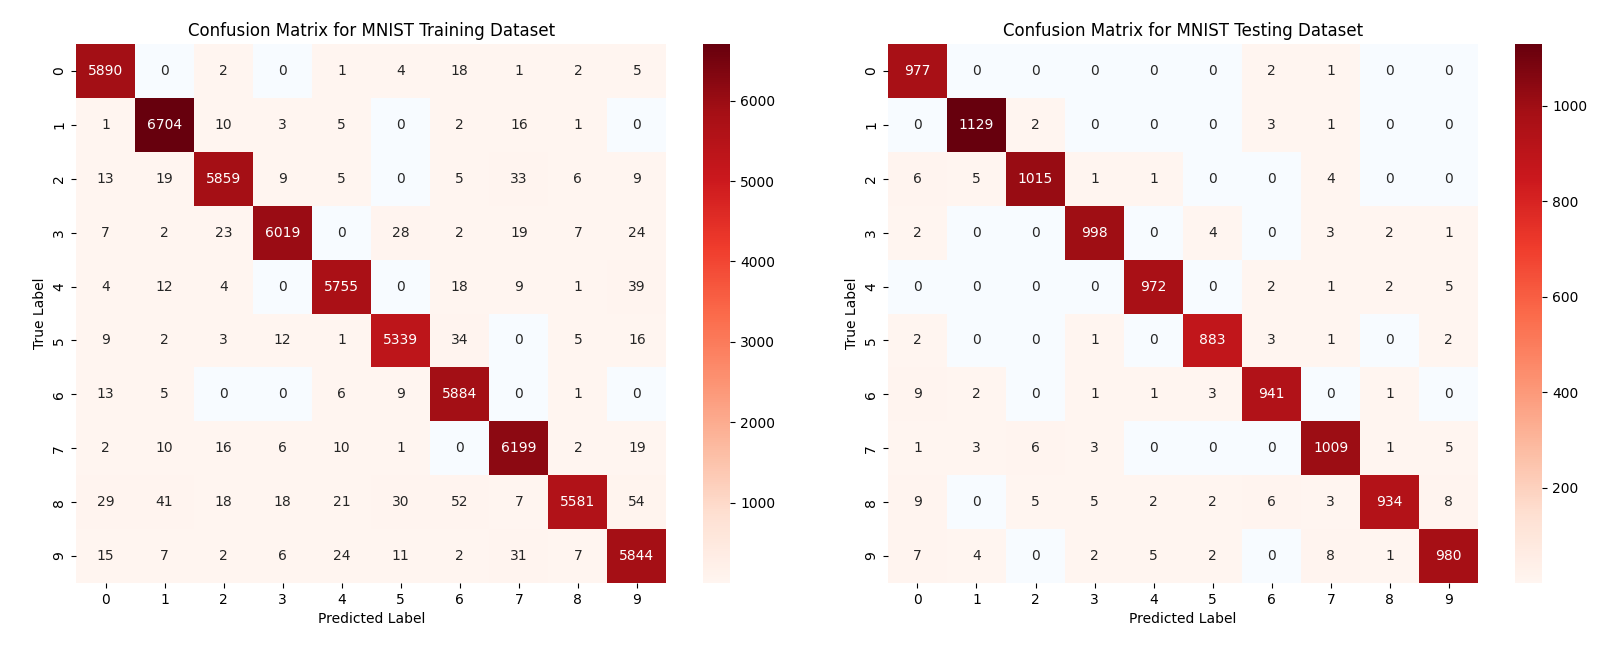
\includegraphics[width=0.99\textwidth]{Figures/Methods/mnist_combined_confusion_matrix.png}
    \caption{Confusion matrices for the MNIST classification model on the training dataset (left) and testing dataset (right). The matrices display the true labels on the vertical axis and the predicted labels on the horizontal axis. The diagonal elements represent correctly classified instances, while the off-diagonal elements indicate misclassifications.}
    \label{fig:mnist_combined_confusion_matrix}
\end{figure}

The accuracy on the training dataset in 98.38\% and 98.46\% on the testing dataset. Figure \ref{fig:mnist_combined_misclassifications}. We note that for both datasets, number zero is the digit less likely, and number eight is the digit most likely to be misclassified. Other digits that are less likely to be misclassified are digits one and; six in the training dataset, and five in the testing dataset. The confusion matrices in Figure \ref{fig:mnist_combined_confusion_matrix} provide some insights into what are the most likely misclassifications, for example digit eight is likely to be misclassified as six or nine, while digit three is likely to be misclassified as two, five or nine.
% For confusion matrices
% [1] Stehman, S. V. (1997). Selecting and interpreting measures of thematic classification accuracy. Remote Sensing of Environment, 62(1), 77-89.

\begin{figure}[h]
    \centering
    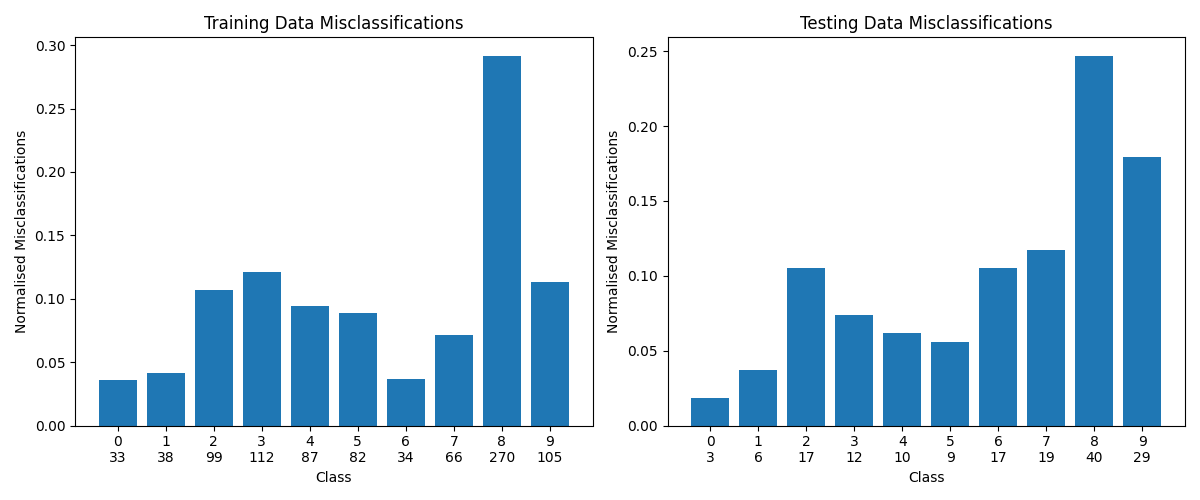
\includegraphics[width=0.99\textwidth]{Figures/Methods/mnist_combined_misclassifications.png}
    \caption{Normalised misclassifications for each class in the training data (left) and testing data (right). The x-axis represents the class labels from 0 to 9, with the corresponding non-normalised misclassification count displayed below each label. The y-axis shows the normalized misclassifications, obtained by dividing the misclassification count for each class by the total number of misclassifications in the respective dataset. }
    \label{fig:mnist_combined_misclassifications}
\end{figure}

\subsection{Clustering}

Clustering algorithms play a crucial role in various domains, enabling the discovery of intrinsic structures and patterns within datasets. These algorithms aim to partition data points into groups or clusters based on their similarity, such that points within the same cluster are more similar to each other than to those in other clusters \citep{jain2010data}. Clustering techniques find applications in a wide range of fields, including image segmentation, anomaly detection, customer segmentation, and bioinformatics \citep{xu2015comprehensive}.

One of the most widely used clustering algorithms is k-means, which iteratively assigns data points to the nearest cluster centroid and updates the centroids based on the assigned points \citep{lloyd1982least}. K-means is computationally efficient and scales well to large datasets, making it suitable for many practical applications. However, it requires specifying the number of clusters in advance and is sensitive to the initial placement of centroids \citep{arthur2007k}.

Another popular clustering approach is hierarchical clustering, which builds a tree-like structure of clusters by either merging smaller clusters into larger ones (agglomerative) or dividing larger clusters into smaller ones (divisive) \citep{johnson1967hierarchical}. Hierarchical clustering provides a visual representation of the clustering process and allows for the exploration of clusters at different granularities. However, it can be computationally expensive and may not scale well to large datasets \citep{mullner2011modern}.

Density-based clustering algorithms, such as DBSCAN (Density-Based Spatial Clustering of Applications with Noise), identify clusters as dense regions separated by areas of lower density \citep{ester1996density}. DBSCAN is particularly useful for detecting clusters of arbitrary shape and handling noise or outliers in the data. It does not require specifying the number of clusters and can discover clusters of varying densities \citep{schubert2017dbscan}.

Clustering algorithms have found numerous applications across various domains. In image segmentation, clustering techniques are used to group pixels with similar characteristics, enabling object detection and recognition \citep{shi2000normalized}. Anomaly detection systems employ clustering to identify unusual patterns or outliers that deviate from the norm, aiding in fraud detection and network intrusion detection \citep{chandola2009anomaly}. Customer segmentation utilizes clustering to group customers with similar behaviors or preferences, facilitating targeted marketing and personalized recommendations \citep{ngai2009application}.

In bioinformatics, clustering algorithms are extensively used for gene expression analysis, protein function prediction, and disease subtype identification \citep{eisen1998cluster}. By grouping genes or proteins with similar expression patterns or functional properties, researchers can gain insights into biological processes and discover potential biomarkers or therapeutic targets \citep{jiang2004cluster}.

The choice of clustering algorithm depends on the specific characteristics of the data, the desired properties of the clusters, and the computational resources available. Researchers continue to develop and improve clustering techniques to address the challenges posed by high-dimensional, large-scale, and complex datasets \citep{rodriguez2019clustering}.

In conclusion, clustering algorithms are essential tools for discovering structures and patterns in data, with applications spanning various domains. From image segmentation and anomaly detection to customer segmentation and bioinformatics, clustering techniques enable researchers and practitioners to extract valuable insights and make data-driven decisions.

To initialise the centroids for K-Means clustering with 10 clusters, where each cluster represents a digit from the MNIST dataset, we leverage the information from the probability distribution of the correct predictions.

The resulting centroids array will have shape (10, 10), where each row represents a centroid for a specific digit. The values in each row correspond to the average probability distribution of the correct predictions for that digit.

To find the centroids, we use:

\begin{algorithm}
\caption{K-Means Centroid Initialisation for MNIST Dataset}
\begin{algorithmic}[1]
\Require{$correct\_preds$: array of shape $(n, 12)$, where $n$ is the number of correct predictions}
\Ensure{$centroids$: array of shape $(10, 10)$, initialised centroids for each digit}

\State $probs\_dist \gets corrects_preds[:, :10]$ \Comment{Extract probability distribution for each digit}
\State $centroids \gets \text{zeros}((10, 10))$ \Comment{Initialise centroids array}

\For{$digit \gets 0$ to $9$}
\State $indices \gets \text{where}(\text{argmax}(probs\_dist, \text{axis}=1) == digit)[0]$ \Comment{Find indices of rows where digit has highest probability}
\State $centroid \gets \text{mean}(probs\_dist[indices], \text{axis}=0)$ \Comment{Compute mean probability distribution for selected rows}
\State $centroids[digit] \gets centroid$ \Comment{Assign centroid to corresponding row in centroids array}
\EndFor

\State \textbf{return} $centroids$
\end{algorithmic}
\end{algorithm}

The algorithm starts with the Require statement, specifying the input correct\_preds array of shape $(n, 12)$, where $n$ is the number of correct predictions.
The Ensure statement specifies the output centroids array of shape $(10, 10)$, which will store the initialised centroids for each digit.
In line 1, we extract the probability distribution for each digit by selecting the first 10 columns of correct\_preds and store it in the prob\_dist array, where column 11 is the label and column 12 is the prediction, and both are the same for correct predictions.
In line 2, we initialise the centroids array with zeros of shape $(10, 10)$ to store the centroid for each digit.
We start a loop that iterates over each digit from 0 to 9.
In line 4, for each digit, we find the indices of rows in prob\_dist where the digit has the highest probability using \text{argmax}(prob\_dist, \text{axis}=1) == digit. This gives us the indices of rows that are most likely to represent the current digit, which is indeed the case since all predictions are correct.
In line 5, we compute the mean probability distribution for the selected rows using \text{mean}(prob\_dist[indices], \text{axis}=0). This gives us the centroid for the current digit.
In line 6, we assign the computed centroid to the corresponding row in the centroids array.
After the loop ends, we return the centroids array.

The resulting centroids array will have shape $(10, 10)$, where each row represents a centroid for a specific digit. The values in each row correspond to the average probability distribution of the correct predictions for that digit.

By initialising the centroids based on the probability distribution of correct predictions, we provide a good starting point for the K-Means algorithm. Each centroid will be initialised to represent the typical probability distribution for a specific digit class prediction, which helps the algorithm converge faster.

Our k-means cluster for 59074 correct MNIST digit predictions converges in a fraction of a second. We then plot the mean distance to centroids for every class in Figure \ref{fig:MNIST_Correct_Training_and_Testing_Mean_Distance_To_Centroids}.

\begin{figure}[h]
    \centering
    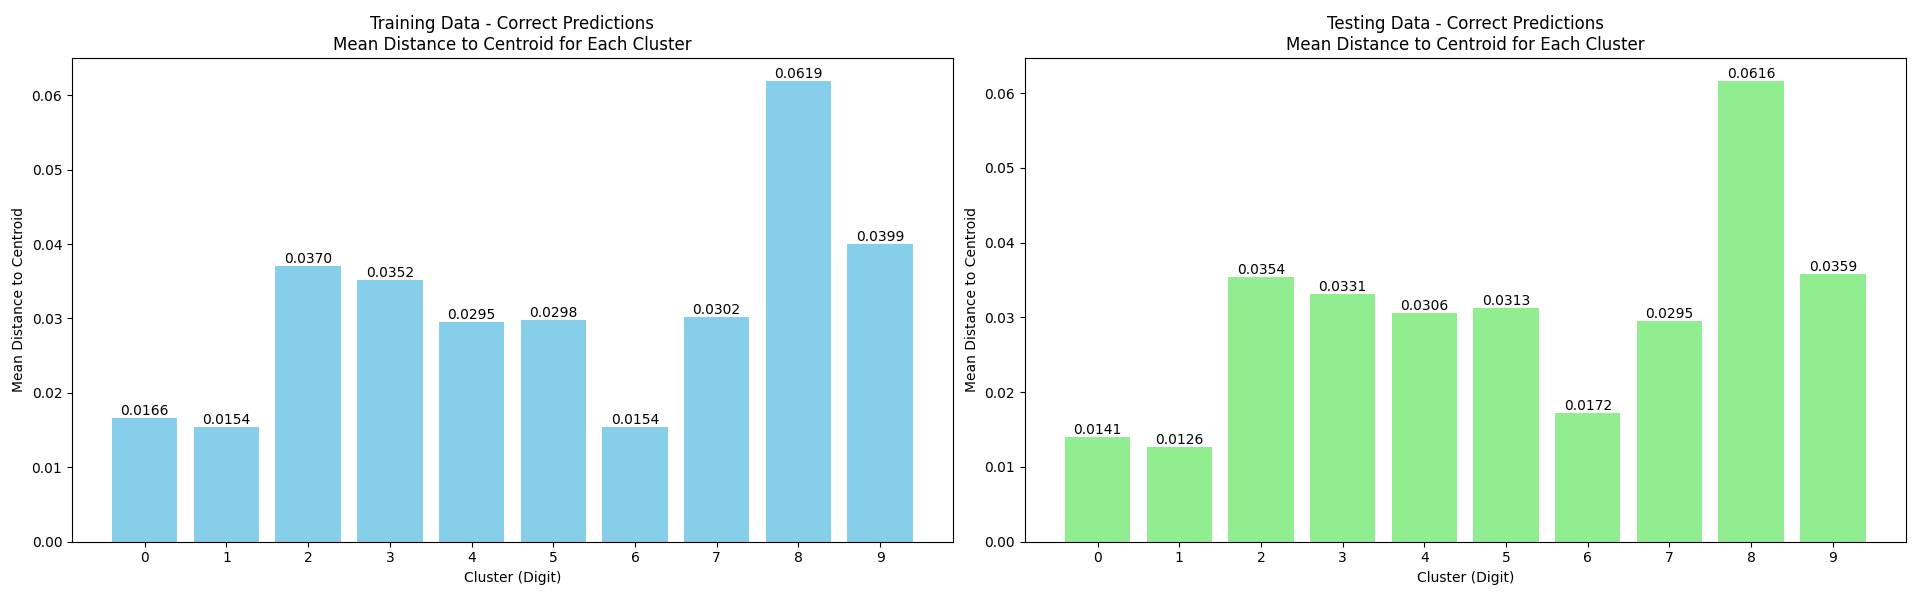
\includegraphics[width=0.99\textwidth]{Figures/Methods/MNIST_Correct_Training_and_Testing_Mean_Distance_To_Centroids.png}
    \caption{Mean distances for Softmax function output for each class, for correct classifications. On the right is the plot for the training dataset and the corresponding test dataset on the right.}
    \label{fig:MNIST_Correct_Training_and_Testing_Mean_Distance_To_Centroids}
\end{figure}

% Function
% plot_mean_distances_double_bars(correct_train_distances, incorrect_train_distances, correct_test_distances, incorrect_test_distances)
% mnist_cnn_eval_saved_softmax_output.py

%% Start claude
The provided figure presents a comparison of the mean distance to centroids for each cluster (digit) between the training data and testing data, considering only the correct predictions. The distance to centroids is a measure of how close the data points (images) are to their respective cluster centers.

Upon analyzing the figure, a key observation emerges: the mean distance to centroids is proportional to the rate of misclassified images for each digit. In other words, digits with a higher number of misclassified images tend to have a larger distance to their corresponding centroids, while digits with fewer misclassifications exhibit smaller distances to their centroids.

Let's take digit 8 as an example. In both the training and testing data, digit 8 stands out as having the highest mean distance to its centroid compared to other digits. This suggests that digit 8 has a relatively higher rate of misclassification, indicating that the model faces more difficulty in accurately recognizing and classifying images of digit 8. The increased distance to the centroid implies that the misclassified images of digit 8 deviate more from the typical representation of that digit.

On the other hand, digits with lower misclassification rates, such as digits 0 and 1, exhibit smaller distances to their respective centroids. This indicates that the model performs better in accurately classifying these digits, and the correctly classified images are more tightly clustered around their centroids.

The proportionality between the mean distance to centroids and the misclassification rate holds true for both the training and testing data, suggesting that this relationship is consistent across different subsets of the dataset.

It's important to note that while the overall pattern of proportionality is evident, there are some variations between the training and testing data. For instance, the mean distances for some digits, like 9 and 6, differ slightly between the two datasets. This could be attributed to differences in the distribution of misclassified images or the presence of outliers in either dataset.

The insights gained from this analysis can be valuable for improving the classification model. By focusing on the digits with higher mean distances to centroids, such as digit 8, researchers can investigate the specific challenges associated with those digits and develop targeted strategies to enhance the model's performance. This may involve collecting more representative training data for those digits, applying data augmentation techniques, or refining the model architecture to better capture the distinctive features of the misclassified images.

In conclusion, the figure highlights the proportional relationship between the mean distance to centroids and the misclassification rate for each digit. Digits with higher misclassification rates exhibit larger distances to their centroids, while digits with fewer misclassifications have smaller distances. This information can guide efforts to improve the classification model's performance by focusing on the digits that pose the greatest challenges.

%% start GPT

The figure presents two bar charts displaying the mean distances from the data points to the centroids of their respective clusters for correctly classified images from the MNIST dataset. The left chart represents the training data, while the right chart corresponds to the testing data. Each bar signifies a cluster that corresponds to a digit from 0 to 9.

Observations from the figure:

1. **Consistency Across Datasets**: Both training and testing data show a similar pattern where certain digits, particularly 1 and 0, have the shortest mean distance to their centroid, indicating that they are, on average, closer to the "ideal" digit representation learned by the model. Conversely, digits such as 8 and 9 have the longest mean distances, suggesting a wider spread of the data points within these clusters.

2. **Distance Proportional to Misclassification Rate**: The charts appear to illustrate a relationship where digits with a greater mean distance to their centroids tend to have a higher rate of misclassification. For instance, digit 8 stands out as having the furthest mean distance in both datasets, which correlates with it having a higher misclassification rate. This suggests that the representations of 8s are more varied or less consistent, leading to less cohesive clustering and, consequently, more frequent misclassifications.

3. **Training vs. Testing Differences**: While the overall trends are similar, some discrepancies between the training and testing datasets can be observed. For example, the mean distance for digit 7 is noticeably higher in the testing data than in the training data. Such differences might imply overfitting or a disparity in the representation of digit 7 between the training and testing subsets.

4. **Implications for Model Improvement**: The digits with the longest distances to centroids could be targets for further investigation and potential improvement of the classification model. This could involve augmenting the training data with more varied examples of these digits or employing techniques like image warping to enhance the robustness of the model to different styles of handwriting.

5. **Data Quality**: The variations in mean distances also reflect the intrinsic quality and diversity of the MNIST data. For example, some digits may inherently have more variability in handwriting styles than others, leading to naturally larger mean distances to centroids.

In summary, the figure effectively communicates key insights into the classifier's performance, highlighting specific digits that may require additional focus for model refinement, potentially guided by the observed mean distance to centroid as an indicator of cluster cohesion and misclassification propensity.

%% Gemini

**Distance to Centroids and Misclassification Rates**

This figure compares the normalized misclassification rates between the training and testing datasets for a Convolutional Neural Network (CNN) model on the MNIST handwritten digit classification task. The x-axis represents the digit classes (0-9). The y-axis shows the normalized misclassification rate, where the height of each bar corresponds to the proportion of images in that class that were misclassified by the model. The teal bars represent the training data, and the orange bars represent the testing data. Text labels at the bottom of each bar indicate the original number of misclassifications for that digit class in the respective dataset.

**Observations**

* **General Trend:** In most digit classes, the misclassification rates are lower in the training data compared to the testing data. This is expected, as the model is trained on the training data and tends to perform better on those examples that it has seen before.
* **Similarity in Patterns:**  Despite the lower overall misclassification rates in training data, the overall pattern of misclassifications (which digits are more prone to errors) appears to be similar between the two datasets. This suggests that the model has learned meaningful features from the training data that generalize well to unseen examples in the testing data.
* **Distance and Misclassification Rates:** The caption mentions a proportional relationship between the distance to centroids and the misclassification rates, however, the visual representation in this specific plot doesn't clearly support that proportionality. While digits 4, 5, 6, and 9 appear to have slightly higher misclassification rates and are further from the center in both datasets, the trend is not entirely consistent across all digits. 

**Possible Explanations**

* **Limited Data:** The distance to centroids might not be the sole factor influencing misclassification rates. Other factors like the inherent complexity of certain digits or the presence of noisy/ambiguous examples within the data can also contribute to misclassifications.
* **Data Visualization:**  The current bar chart might not effectively convey the relationship between distance and misclassification rates. Consider alternative visualizations like scatter plots or overlaid line charts to explore this relationship further.

**Further Analysis**

* **Centroid Visualization:** It would be helpful to visualize the centroids themselves, perhaps using dimensionality reduction techniques to project them into a 2D or 3D space. This could aid in understanding how the centroids are positioned relative to each other and how digit classes are mapped in the feature space. 
* **Class-Specific Analysis:**  Delving deeper into specific digit classes (particularly those with higher misclassification rates) could reveal patterns or properties that make them more challenging for the model.

In Figure \ref{fig:MNIST_Incorrect_Training_and_Testing_Mean_Distance_To_Centroids}, the mean distances for Softmax output for each incorrectly predicted class.

\begin{figure}[h]
    \centering
    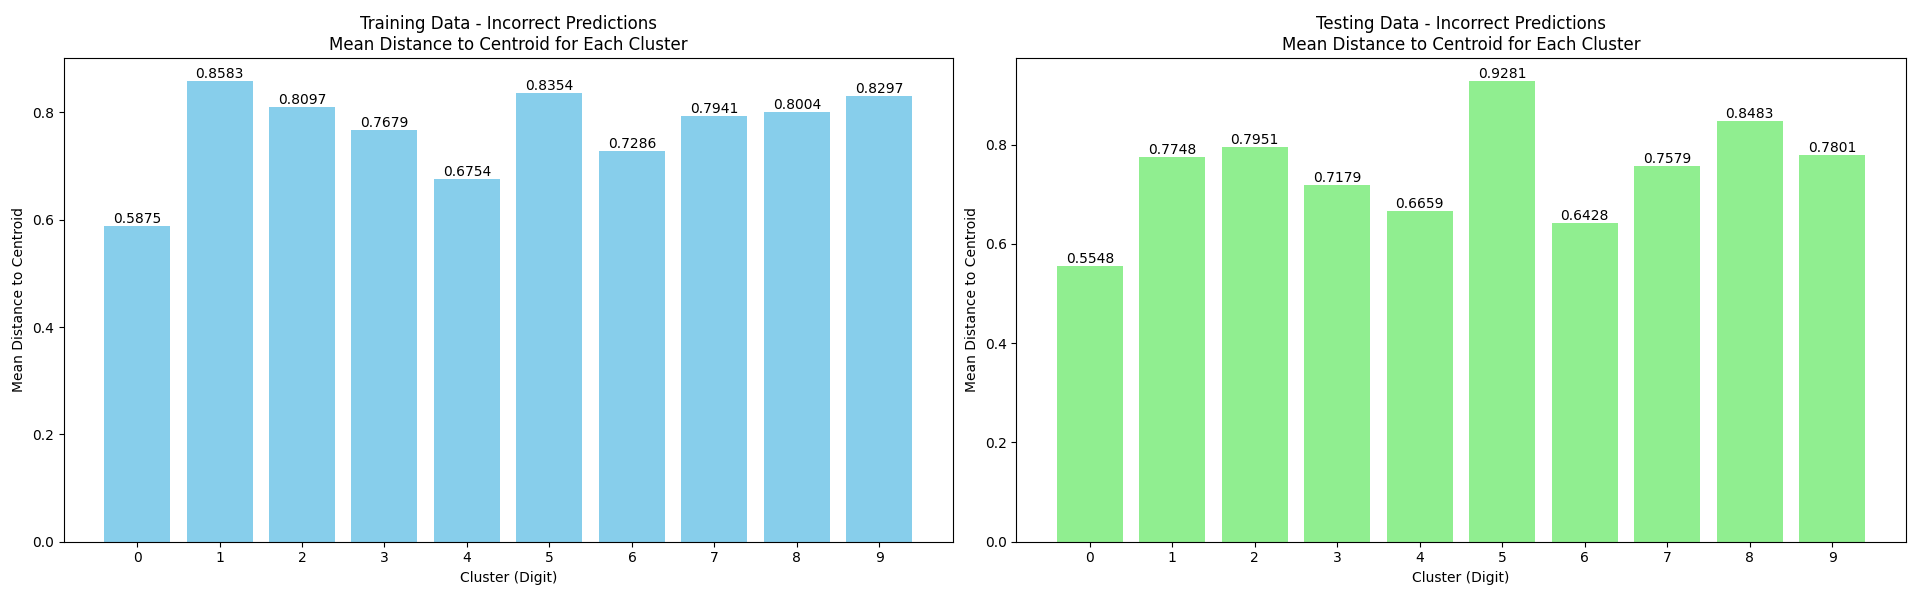
\includegraphics[width=0.99\textwidth]{Figures/Methods/MNIST_Incorrect_Training_and_Testing_Mean_Distance_To_Centroids.png}
    \caption{Mean distances for Softmax function output for each class, for incorrect classifications. On the right is the plot for the training dataset and the corresponding test dataset on the right.}
    \label{fig:MNIST_Incorrect_Training_and_Testing_Mean_Distance_To_Centroids}
\end{figure}

% Claude

The figure presents the mean distance to centroids for each cluster (digit) in the training and testing data, focusing on incorrect predictions. The analysis reveals a notable trend: digits with higher misclassification rates exhibit larger distances to their respective centroids, indicating a greater deviation from the typical representation of those digits.

In both datasets, digits 8 and 9 stand out with the highest mean distances to their centroids, suggesting a higher prevalence of misclassifications. This implies that the model struggles to accurately classify images of these digits, leading to a greater spread of misclassified instances around the cluster centers.

Conversely, digits with lower misclassification rates, such as 0 and 6 in the training data and 1 and 5 in the testing data, display smaller distances to their centroids. This indicates that even among the misclassified instances, these digits maintain a relatively closer proximity to their cluster centers, reflecting a lower degree of deviation.

Interestingly, while the overall pattern of proportionality between misclassification rates and centroid distances holds true, there are notable differences between the training and testing data. For instance, digit 5 exhibits a higher mean distance in the training data compared to the testing data, suggesting potential variations in the distribution of misclassified instances across the datasets.

These findings highlight the importance of focusing on the digits with larger centroid distances, as they represent the most challenging cases for the classification model. By investigating the specific characteristics and patterns of misclassified instances for these digits, researchers can gain valuable insights into the model's limitations and develop targeted strategies to enhance its performance.

In summary, the figure reveals a proportional relationship between the mean distance to centroids and the misclassification rates for each digit, with higher misclassification rates corresponding to larger centroid distances. This information can guide efforts to improve the model's accuracy by addressing the specific challenges associated with the most problematic digits.

% GPT

Figure Z illustrates the mean distance to centroid for each cluster corresponding to MNIST dataset digits, specifically for incorrect classifications within both training (left) and testing (right) datasets. The mean distance serves as a proxy for the dissimilarity of misclassified instances from the cluster centroid, with higher values indicating greater deviation from the archetype of each respective digit's cluster.

The chart evidences that misclassified digits tend to have a markedly higher mean distance to their respective centroids compared to correctly classified instances, as expected. Digits such as '1' and '0' in the training set and '1' in the testing set manifest the smallest mean distances, implying a tighter cluster formation even amongst misclassified samples. Conversely, digit '8' in the testing set exhibits the largest mean distance, indicative of the greatest variation from the cluster centroid and, by extension, the highest level of heterogeneity within its misclassified samples. 

This disparity in mean distances underscores the variability inherent in certain digits' representation, suggesting avenues for further model refinement. Enhancements in feature extraction and the application of more sophisticated clustering algorithms may reduce these distances and improve classification accuracy.

Figure \ref{fig:MNIST_Correct_and_Incorrect_Training_and_Testing_Mean_Distance_To_Centroids} shows the plots side by side.

\begin{figure}[h]
    \centering
    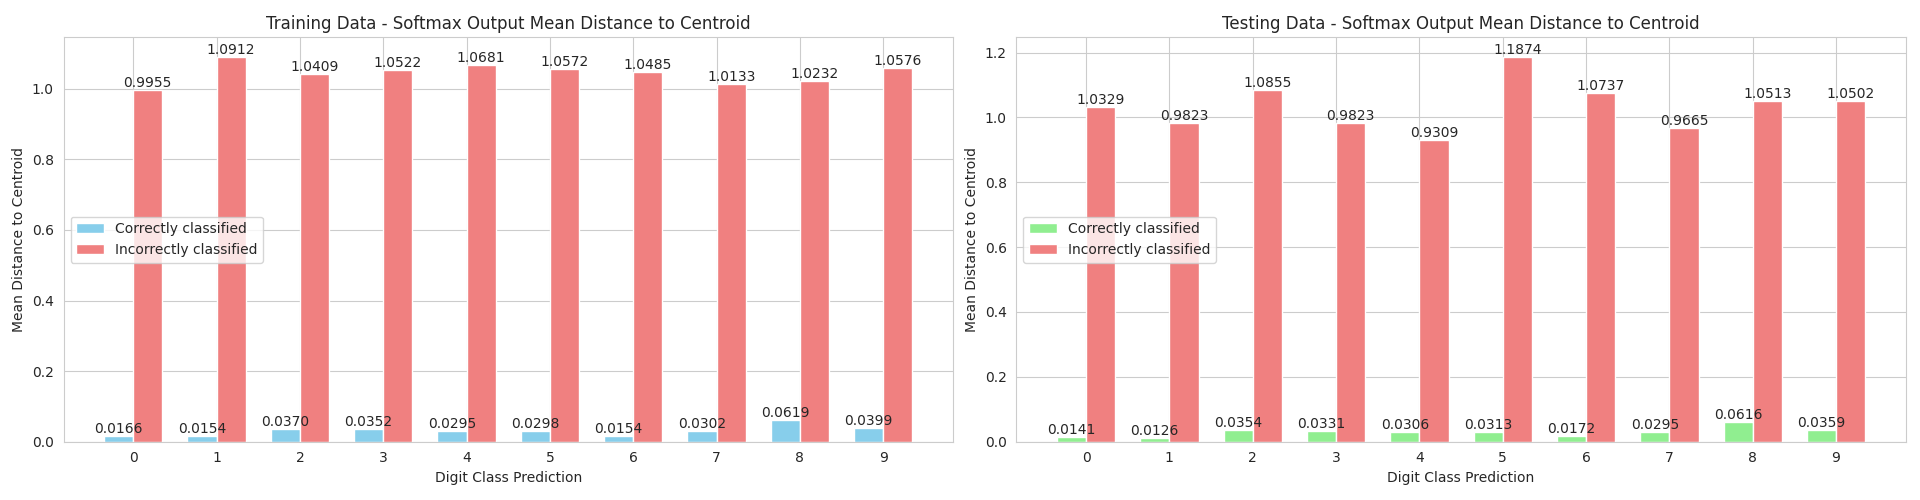
\includegraphics[width=0.99\textwidth]{Figures/Methods/MNIST_Correct_and_Incorrect_Training_and_Testing_Mean_Distance_To_Centroids.png}
    \caption{Mean distances for Softmax function output for each class, for incorrect classifications. On the right is the plot for the training dataset and the corresponding test dataset on the right.}
    \label{fig:MNIST_Correct_and_Incorrect_Training_and_Testing_Mean_Distance_To_Centroids}
\end{figure}

The plots in Figure \ref{fig:boxplots_side_by_side_x2} compare the distribution of distances to centroids for correctly and incorrectly classified instances across different digit classes in both the training and testing MNIST datasets.

In the training data (left plot), the distances for correctly classified instances are lower than those of incorrectly classified instances across all digit classes. This indicates that the distance of the Softmax output to the K-Means cluster centroids are good candidate proxies for accuracy, leading to smaller distances for correct classifications.

\begin{figure}[h]
    \centering
    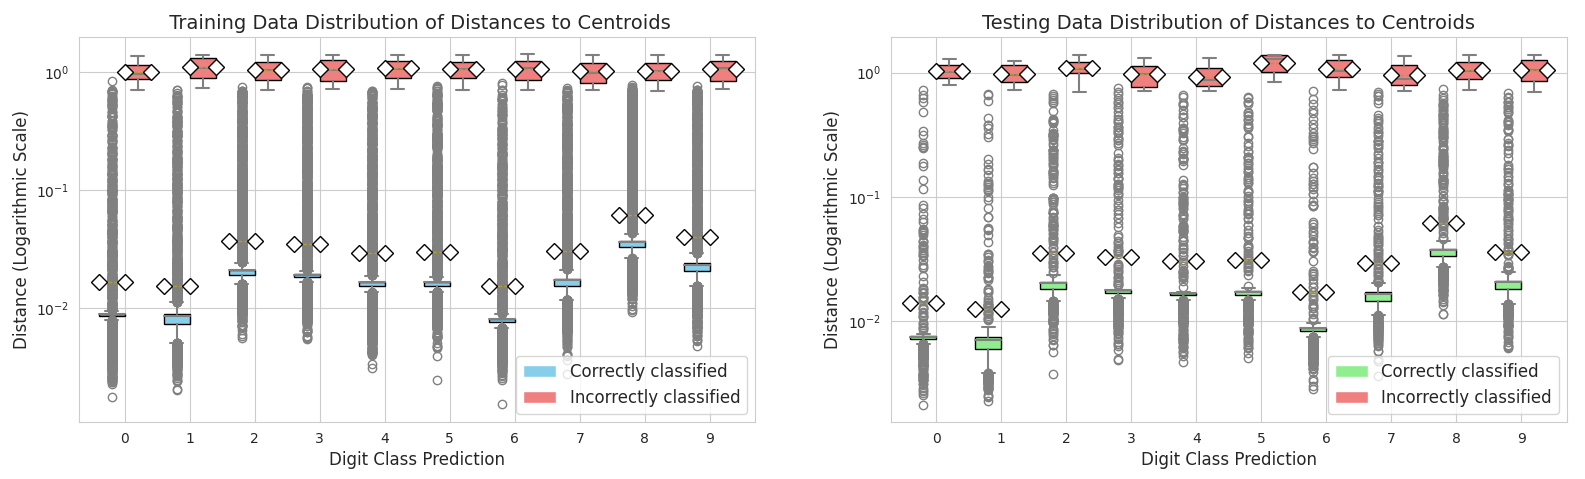
\includegraphics[width=0.99\textwidth]{Figures/Methods/boxplots_side_by_side_x2.png}
    \caption{Distribution of Distances to Centroids for Correctly and Incorrectly Classified Instances in Training and Testing MNIST Data, where training data is on the left and testing data is displayed on the right. Distances are shown on a logarithmic scale.}
    \label{fig:boxplots_side_by_side_x2}
\end{figure}


% Plot generated with function call:
% plot_mean_distances_double_bars(correct_train_distances, incorrect_train_distances, correct_test_distances, incorrect_test_distances, save=True)

\begin{table}[h]
\centering
\scriptsize
\begin{tabular}{c|cccccc|cccccc}
\hline
 & \multicolumn{6}{c|}{Training Dataset Correct Predictions} & \multicolumn{6}{c}{Training Dataset Incorrect Predictions} \\
Index & Mean & Median & Min & Max & $\sigma$ & Count & Mean & Median & Min & Max & $\sigma$ & Count \\ \hline
0 & 0.0166 & 0.0088 & 0.0018 & 0.8433 & 0.0536 & 5890 & 0.9955 & 0.9552 & 0.7037 & 1.3681 & 0.1756 & 33 \\
1 & 0.0154 & 0.0085 & 0.0020 & 0.7051 & 0.0486 & 6704 & 1.0912 & 1.0771 & 0.7247 & 1.3909 & 0.2197 & 38 \\
2 & 0.0370 & 0.0208 & 0.0056 & 0.7453 & 0.0746 & 5859 & 1.0409 & 1.0460 & 0.6962 & 1.3912 & 0.2064 & 99 \\
3 & 0.0352 & 0.0192 & 0.0055 & 0.7509 & 0.0754 & 6019 & 1.0522 & 1.0338 & 0.7139 & 1.3999 & 0.2143 & 112 \\
4 & 0.0295 & 0.0166 & 0.0031 & 0.6933 & 0.0661 & 5755 & 1.0681 & 1.0642 & 0.7139 & 1.4010 & 0.2045 & 87 \\
5 & 0.0298 & 0.0165 & 0.0024 & 0.7634 & 0.0693 & 5339 & 1.0572 & 1.0560 & 0.7066 & 1.3956 & 0.2000 & 82 \\
6 & 0.0154 & 0.0081 & 0.0015 & 0.7981 & 0.0485 & 5884 & 1.0485 & 1.0702 & 0.7068 & 1.4015 & 0.2110 & 34 \\
7 & 0.0302 & 0.0171 & 0.0028 & 0.7365 & 0.0678 & 6199 & 1.0133 & 0.9764 & 0.6960 & 1.3989 & 0.2160 & 66 \\
8 & 0.0619 & 0.0363 & 0.0092 & 0.7788 & 0.0989 & 5581 & 1.0232 & 1.0083 & 0.6852 & 1.3816 & 0.1990 & 270 \\
9 & 0.0399 & 0.0232 & 0.0048 & 0.7616 & 0.0781 & 5844 & 1.0576 & 1.0830 & 0.7179 & 1.3974 & 0.2201 & 105 \\ \hline
 & \multicolumn{6}{c|}{Testing Dataset Correct Predictions} & \multicolumn{6}{c}{Testing Dataset Incorrect Predictions} \\
Index & Mean & Median & Min & Max & $\sigma$ & Count & Mean & Median & Min & Max & $\sigma$ & Count \\ \hline
0 & 0.0141 & 0.0075 & 0.0021 & 0.7225 & 0.0506 & 977 & 1.0329 & 1.0185 & 0.7923 & 1.2880 & 0.2026 & 3 \\
1 & 0.0126 & 0.0071 & 0.0023 & 0.6737 & 0.0445 & 1129 & 0.9823 & 0.9556 & 0.7278 & 1.2445 & 0.1898 & 6 \\
2 & 0.0354 & 0.0202 & 0.0037 & 0.6697 & 0.0704 & 1015 & 1.0855 & 1.0725 & 0.7010 & 1.3833 & 0.1844 & 17 \\
3 & 0.0331 & 0.0177 & 0.0049 & 0.7515 & 0.0765 & 998 & 0.9823 & 0.9752 & 0.7102 & 1.3230 & 0.2044 & 12 \\
4 & 0.0306 & 0.0169 & 0.0047 & 0.6603 & 0.0678 & 972 & 0.9309 & 0.8725 & 0.7073 & 1.3110 & 0.1923 & 10 \\
5 & 0.0313 & 0.0173 & 0.0051 & 0.6324 & 0.0692 & 883 & 1.1874 & 1.2976 & 0.8477 & 1.3982 & 0.2067 & 9 \\
6 & 0.0172 & 0.0088 & 0.0029 & 0.7135 & 0.0545 & 941 & 1.0737 & 1.0242 & 0.7240 & 1.4009 & 0.2120 & 17 \\
7 & 0.0295 & 0.0165 & 0.0036 & 0.6939 & 0.0678 & 1009 & 0.9665 & 0.8833 & 0.7148 & 1.3628 & 0.2016 & 19 \\
8 & 0.0616 & 0.0372 & 0.0114 & 0.7328 & 0.0918 & 934 & 1.0513 & 1.0399 & 0.7252 & 1.3842 & 0.2022 & 40 \\
9 & 0.0359 & 0.0206 & 0.0042 & 0.6870 & 0.0765 & 980 & 1.0502 & 1.0486 & 0.6968 & 1.3838 & 0.2197 & 29 \\ \hline
\end{tabular}
\caption{Statistical Summary of MNIST Softmax Output Distances to Centroids for Different Datasets and Prediction Outcomes. The centroids are obtained with Softmax outputs for correct predictions from the training and testing datasets.}
\label{tab:distance_to_centroid}
\end{table}

% DATA for table above
%        Mean    Median       Min       Max  Standard Deviation  Count
% 0  0.016608  0.008843  0.001769  0.843304            0.053614   5890
% 1  0.015435  0.008516  0.002036  0.705149            0.048557   6704
% 2  0.036996  0.020828  0.005605  0.745250            0.074615   5859
% 3  0.035151  0.019205  0.005478  0.750860            0.075377   6019
% 4  0.029493  0.016613  0.003111  0.693346            0.066094   5755
% 5  0.029819  0.016509  0.002448  0.763396            0.069287   5339
% 6  0.015405  0.008078  0.001526  0.798075            0.048491   5884
% 7  0.030247  0.017138  0.002791  0.736508            0.067780   6199
% 8  0.061884  0.036283  0.009184  0.778795            0.098932   5581
% 9  0.039943  0.023188  0.004768  0.761636            0.078053   5844
%        Mean    Median       Min       Max  Standard Deviation  Count
% 0  0.995516  0.955230  0.703653  1.368133            0.175639     33
% 1  1.091157  1.077065  0.724706  1.390934            0.219724     38
% 2  1.040888  1.046023  0.696177  1.391211            0.206378     99
% 3  1.052159  1.033801  0.713948  1.399858            0.214313    112
% 4  1.068138  1.064157  0.713896  1.400997            0.204490     87
% 5  1.057245  1.055964  0.706555  1.395563            0.200003     82
% 6  1.048483  1.070162  0.706828  1.401450            0.211018     34
% 7  1.013332  0.976427  0.695997  1.398902            0.216013     66
% 8  1.023217  1.008262  0.685179  1.381630            0.199017    270
% 9  1.057626  1.082991  0.717850  1.397425            0.220102    105
%        Mean    Median       Min       Max  Standard Deviation  Count
% 0  0.014064  0.007518  0.002131  0.722502            0.050551    977
% 1  0.012627  0.007062  0.002254  0.673694            0.044504   1129
% 2  0.035369  0.020174  0.003719  0.669724            0.070428   1015
% 3  0.033119  0.017744  0.004876  0.751473            0.076455    998
% 4  0.030573  0.016858  0.004709  0.660308            0.067756    972
% 5  0.031271  0.017275  0.005053  0.632375            0.069207    883
% 6  0.017175  0.008774  0.002851  0.713528            0.054455    941
% 7  0.029476  0.016466  0.003639  0.693906            0.067756   1009
% 8  0.061609  0.037214  0.011389  0.732832            0.091848    934
% 9  0.035850  0.020602  0.004236  0.686980            0.076507    980
%        Mean    Median       Min       Max  Standard Deviation  Count
% 0  1.032918  1.018475  0.792297  1.287982            0.202620      3
% 1  0.982310  0.955644  0.727825  1.244521            0.189784      6
% 2  1.085502  1.072510  0.700976  1.383269            0.184444     17
% 3  0.982309  0.975231  0.710249  1.322951            0.204446     12
% 4  0.930852  0.872484  0.707302  1.310962            0.192325     10
% 5  1.187412  1.297633  0.847685  1.398223            0.206653      9
% 6  1.073695  1.024168  0.724028  1.400876            0.211957     17
% 7  0.966459  0.883283  0.714793  1.362762            0.201621     19
% 8  1.051282  1.039866  0.725232  1.384221            0.202232     40
% 9  1.050175  1.048609  0.696760  1.383811            0.219746     29
% TODO Boxplots

Figure \ref{fig:MNIST_Classification_Train_Test_Accuracy_Mean_Distance_to_Centroid_Linear_Fit} shows the linear fit for Accuracy and Mean Class Distances to Centroids.

In the context of the MNIST dataset, the derived linear functions from the training and testing data exhibit a negative correlation between the classification accuracy and the mean class distances to the centroids. Specifically, the training data is described by the function $ y = -0.806x + 1.009 $, and the testing data by $ y = -0.677x + 1.004 $. The negative coefficients of the linear terms $ -0.806 $ and $ -0.677 $, respectively) indicate that an increase in the mean distance to the centroid correlates with a decrease in classification accuracy for both datasets.

These results suggest a clear inverse relationship: as the mean distance from the data points in a class to their centroid increases, the propensity for correct classification diminishes. This could be due to the spread of data points within a class – greater distances from the centroid reflect a larger variance within the class, potentially making it more challenging for the classifier to identify the defining characteristics of each class accurately.

The steeper slope for the training data function implies that accuracy is more sensitive to changes in mean distance to centroid during training. Conversely, the testing data's function has a less steep slope, which could suggest that the classifier is slightly more robust to variation in the testing set, or that the testing set has inherently less variation in mean distances across classes.

\begin{figure}[h]
    \centering
    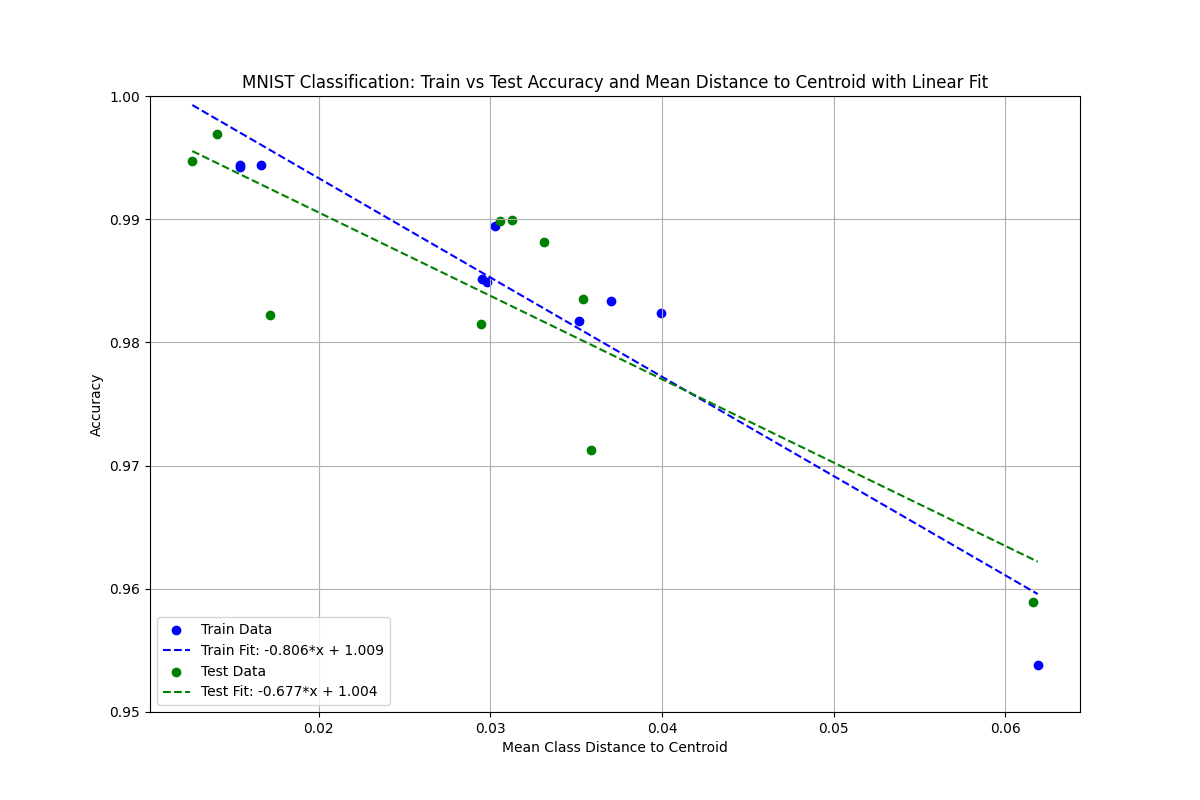
\includegraphics[width=0.99\textwidth]{Figures/Methods/MNIST_Classification_Train_Test_Accuracy_Mean_Distance_to_Centroid_Linear_Fit.png}
    \caption{Scatter plot depicting the relationship between classification accuracy and mean class distance to the centroid for the MNIST dataset. Training data (blue dots) and testing data (green dots) are each fitted with a linear regression line, demonstrating a negative correlation where increased mean distance corresponds to decreased accuracy. The steeper slope of the training data fit (-0.806) compared to the testing data fit (-0.677) reflects the greater accuracy and more compact cluster obtained from the correct test predictions compared to the cluster obtained from correct training predictions.}
    \label{fig:MNIST_Classification_Train_Test_Accuracy_Mean_Distance_to_Centroid_Linear_Fit}
\end{figure}

% function call
% plot_digit_averages(train_correct_predictions, train_incorrect_predictions, color1='skyblue', color2='lightcoral', data="Training Data")

\begin{figure}[h]
    \centering
    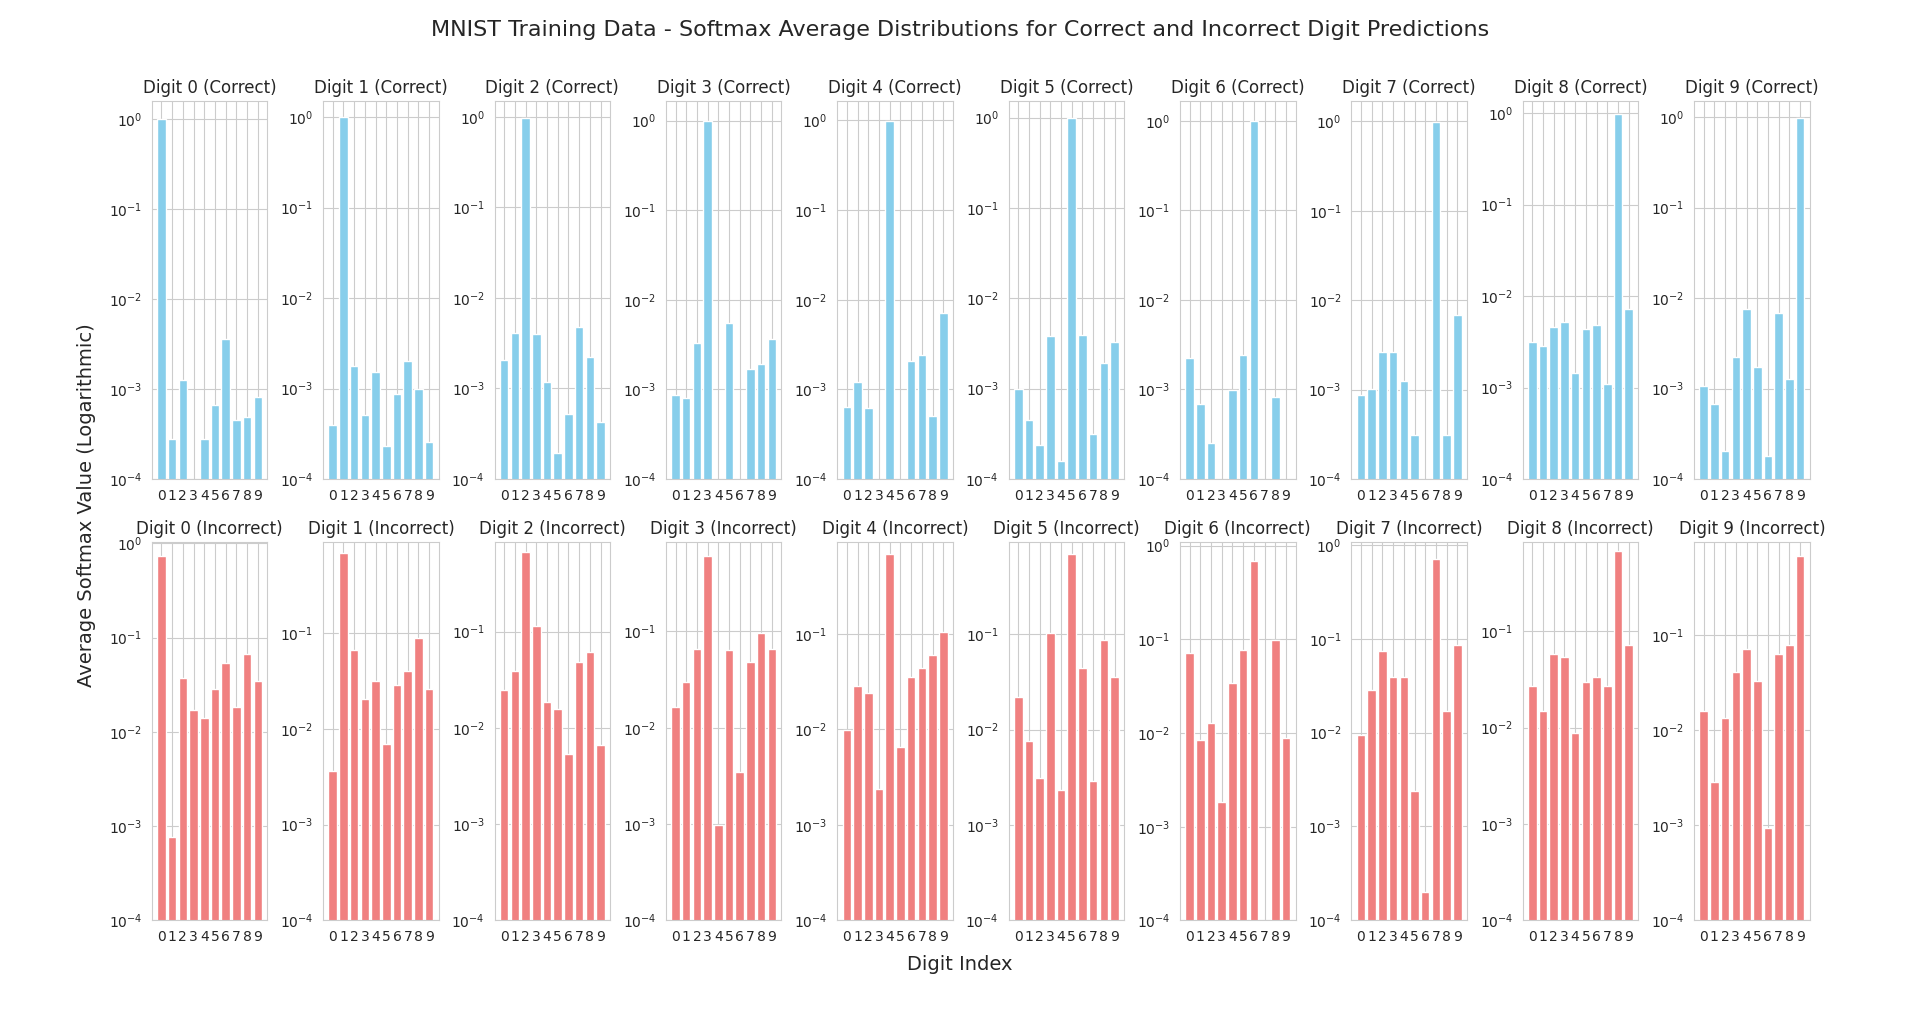
\includegraphics[width=0.99\textwidth]{Figures/Methods/MNIST_Softmax_Averages_Training.png}
    \caption{Average Softmax Probabilities for Correctly and Incorrectly Classified Digits in the MNIST Training Dataset}
    \label{fig:MNIST_Softmax_Averages_Training}
\end{figure}

% Plot generated with function:
% plot_accuracy_vs_distance_linear_fit(correct_train_distances, train_class_accuracies, correct_test_distances, test_class_accuracies)
% mnist_cnn_eval_saved_softmax_output.py

% Both fits reinforce the concept that compact clusters lead to better classification performance. ???
% Do they ???

These insights are crucial for informing the refinement of the classification model. They indicate that efforts to reduce within-class variance, potentially through data augmentation or more sophisticated feature extraction, could result in improved accuracy. Furthermore, understanding the different sensitivities in training versus testing can help diagnose overfitting and guide the development of more generalisable models.

In summary, the linear relationship elucidated by the fitted functions provides quantitative backing for the intuitive notion that tighter clusters (with respect to the centroid) lead to better classification performance. It reinforces the importance of cluster cohesion as an objective metric in assessing and improving classifier models, particularly in the realm of handwritten digit recognition.

% d2c = calculate_distances_to_centroids(train_correct_predictions, centroids)
% uel, ucnts = np.unique(d2c[:, 1], return_counts=True)
% ucnts
% array([5890, 6704, 5859, 6019, 5755, 5339, 5884, 6199, 5581, 5844])

Figure \ref{fig:MNIST_Softmax_Averages_Training} shows the average softmax probabilities for each digit class (0 to 9) in the MNIST training dataset, separated into correctly classified instances (top row) and incorrectly classified instances (bottom row). The probabilities are displayed on a logarithmic scale. For correctly classified digits, the highest average probability is observed for the corresponding true digit class, indicating strong confidence in the correct predictions. In contrast, for incorrectly classified digits, the average probabilities are more evenly distributed across different digit classes, suggesting lower confidence and potential confusion between similar-looking digits. The plot provides insights into the model's behavior and the challenges in accurately classifying certain digit classes.
Figure \ref{fig:MNIST_Softmax_Averages_Testing} is the corresponding plot for the MNIST testing dataset.

% function call
% plot_digit_averages(test_correct_predictions, test_incorrect_predictions, color1='lightgreen', color2='lightcoral', data="Testing Data")
\begin{figure}[h]
    \centering
    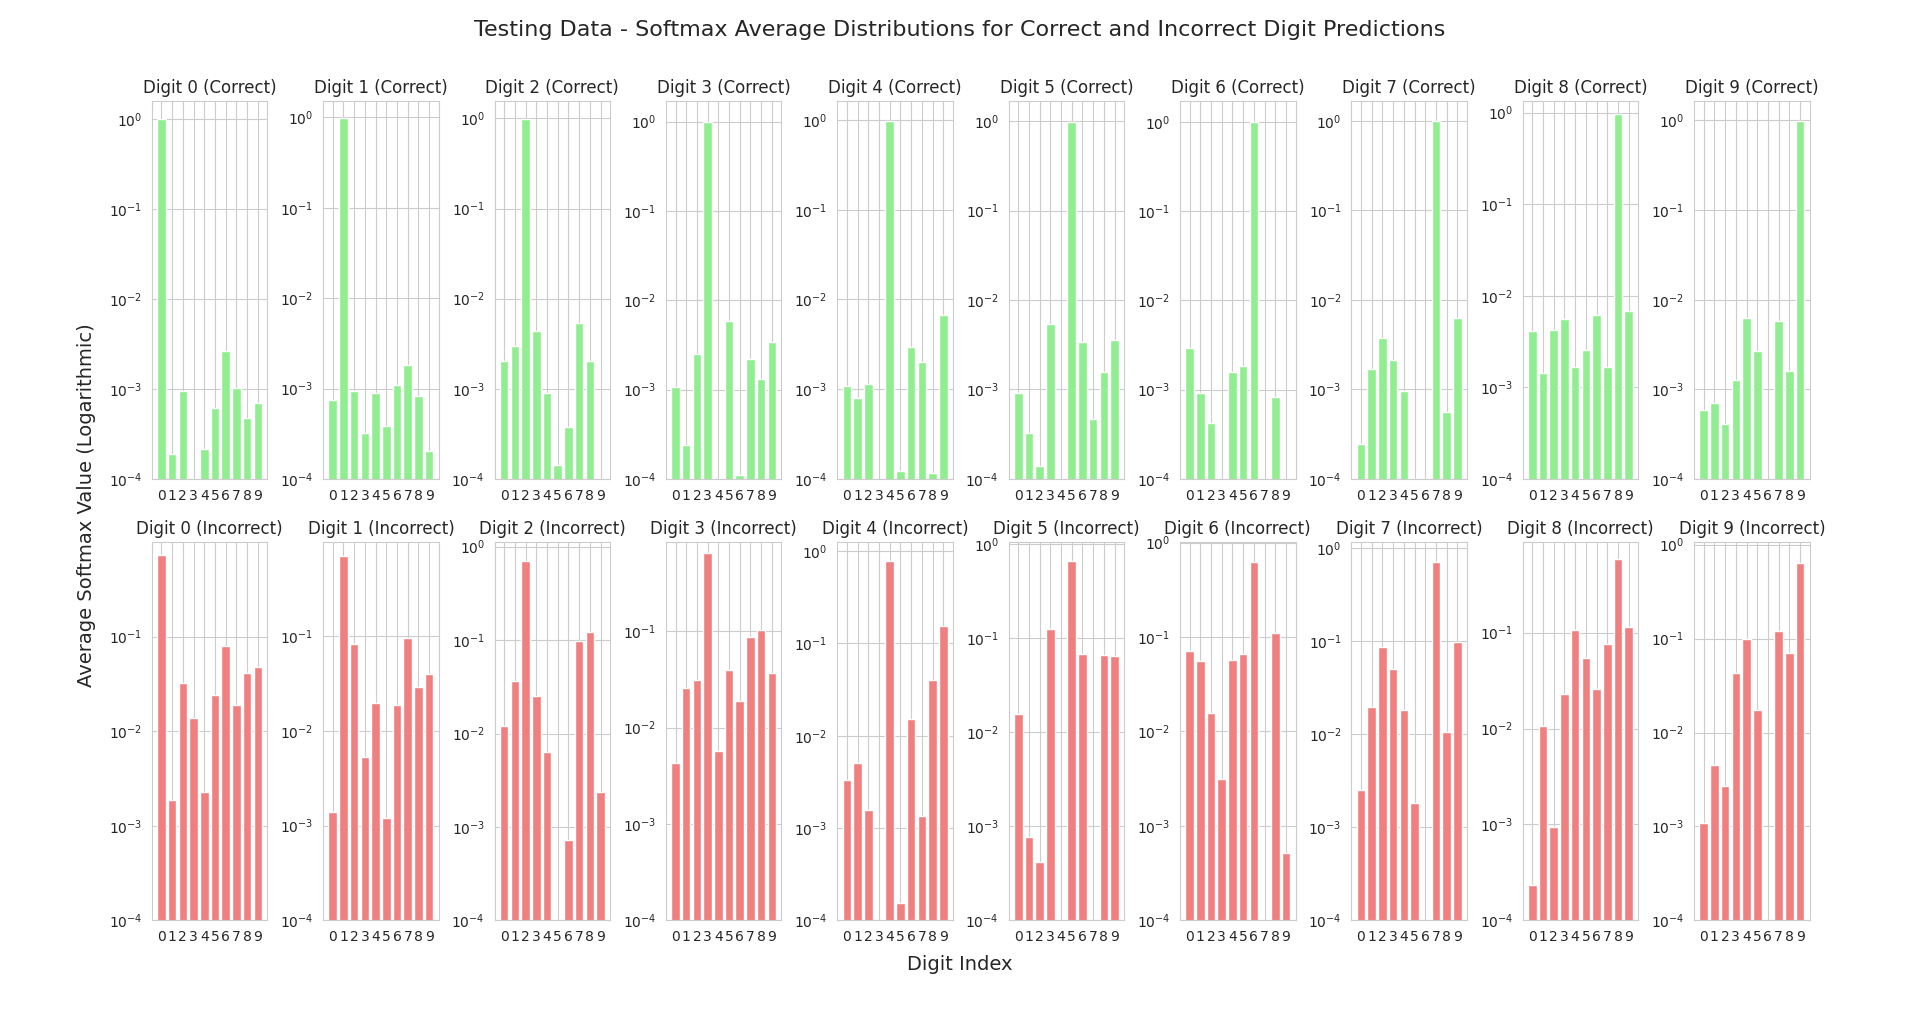
\includegraphics[width=0.99\textwidth]{Figures/Methods/MNIST_Softmax_Averages_Testing.png}
    \caption{Average Softmax Probabilities for Correctly and Incorrectly Classified Digits in the MNIST Testing Dataset.}
    \label{fig:MNIST_Softmax_Averages_Testing}
\end{figure}


The maximum distance between two points in an n-dimensional space depends on the constraints applied to the coordinates. For probability distributions, each coordinate must be non-negative, and the sum of all coordinates must equal 1. These constraints define a simplex in the n-dimensional space. For a vector $\mathbf{p} = (p_1, ..., p_n)$ in this space:

\begin{equation}
\sum_{i=1}^n p_i = 1 \quad \text{and} \quad p_i \geq 0 \quad \forall i
\end{equation}

The maximum Euclidean distance between two points in this simplex occurs between vertices. Each vertex has one coordinate equal to 1 and all others equal to 0. The Euclidean distance $d$ between two vertices $\mathbf{p}$ and $\mathbf{q}$ is:

\begin{equation}
d(\mathbf{p}, \mathbf{q}) = \sqrt{\sum_{i=1}^n (p_i - q_i)^2}
\end{equation}

For two vertices that differ in positions $j$ and $k$, we have $p_j = 1$, $q_j = 0$, $p_k = 0$, $q_k = 1$, and all other coordinates are 0. This gives:

\begin{equation}
d(\mathbf{p}, \mathbf{q}) = \sqrt{(1-0)^2 + (0-1)^2} = \sqrt{2}
\end{equation}

This maximum distance applies to neural networks with softmax outputs. A prediction for class $j$ produces a vector with maximum probability at position $j$. When the network assigns probability 1 to a class, the output is a vertex of the simplex. The distance between predictions of different classes reaches its maximum of $\sqrt{2}$ when the network assigns probability 1 to each class.


\subsection{Perturbed MNIST testing dataset}

We "perturb" the MNIST testing dataset with 12 different types of noise at 10 levels, that is an additional 120 images created for every image. The original testing dataset consists of 10,000 examples. With the perturbations, the total comes to 1,210,000. We store the perturbed images in file 't1210k-perturbed-images-idx3-ubyte', the labels in file 't1210k-perturbed-labels-idx1-ubyte', and the perturbation levels in file 't1210k-perturbation-levels-idx0-ubyte'. The files are generated by script generate\_pmnist\_dataset.py, in repository https://github.com/dsikar/pmnist.git. 
We then use script mnist\_cnn\_eval\_perturbed\_softmax\_output.py to make a prediction for every image in 't1210k-perturbed-images-idx3-ubyte', storing the true label, predicted label, perturbation type and level, to further study the change in distance to centroid as a result of added noise, and also compare metrics KL, DB and HI with the distance to centroid.

Next we use the Vanilla CNN to generate the softmax probabilities. In a first pass, we store the softmax probabilities, the true label, the predicted label, the perturbation type and the perturbation intensity resulting in a $(n,14)$ dimensional array.

We also store the centroids in a $(10,10)$ array.

On a second pass we iterate though all the images in 't1210k-perturbed-images-idx3-ubyte' and add another 4 values:

\begin{enumerate}
    \item Distance to centroid
    \item Bhattacharya Distance of perturbed image to original image
    \item Histogram Intersection of perturbed image to original image
    \item KL Divergence of perturbed image to original image
\end{enumerate}

Noting that Bhattacharya Distance, Histogram Intersection and KL Divergence from original image to itself will be 0, 1 and 0 respectively.

We are interested in observing how the the distance to centroid quantity correlates to the Bhattacharya Distance, Histogram Intersection and KL Divergence quantities. Since 12 distinct perturbation types are applied, at 10 distinct levels, we group by perturbation type and plot the perturbation level as the independent variable, and each of the distances as the dependent variable, for each class, then for all classes combined. The expectation is that BD, KL and distance to centroid will be positive correlated to increase in noise, whereas HI will be negatively correlated to increase in noise (less means further away from original image in this case).

We aggregate the data in a single array of dimensions $(n,18)$ where $n$ is the number of rows, the first 10 columns are the softmax output of the image label prediction, column 11 is the label, column 12 is the prediction, column 13 is the perturbation type, column 14 is the perturbation level, column 15 is the Bhattacharya distance between the perturbed image and the original image, column 16 is the Histogram Intersection and column 17 is the KL divergence. Note, for the original image, the BD, HI and KL are 0, 1 and 0, as we are comparing an image to itself.

We show 48 plots in groups of 12 * 4

%4 (distance metrics) x 12 (types of noise) = 48 plots

We compare cluster proximity 2 clusters at a time in a confusion matrix. We notice that as the error increases, the overlap between clusters also increases. 2D clusters

Other options for distance metrics exist including, and not limited to, BD, KL, E, CS - cite table in results.

\subsection{Generating Softmax Outputs, Centroids, for Self-Driving}

Qwen model:
See experiments 278 for determining token IDs and 279 for extracting softmax outputs

Then the workflow is:

\subsection{VLM Remote Inference}
The process involves three scripts for vision-based vehicle steering predictions. A remote inference script on a high-performance computing cluster monitors an input directory for .jpg images from the simulator’s front-facing camera, performs inference, and saves softmax outputs as .npy files in a remote output directory. A local broker script continuously transfers .jpg images from a local input directory to the remote input directory and .npy files from the remote output directory to a local output directory. The local simulation script generates camera images, places them in the local input directory, retrieves softmax predictions, and applies steering to the simulated vehicle. Technical details are provided in Appendix %~\ref{app:technical_details}. % COMMENT IN WHEN COMPILING WITH APPENDIX

% How to best structure ?
% One possibility
% Datasets
% | pminist
% | cifar10
% | carla self driving - continuous
% | carla self driving - continuous with fiducials
% | carla self driving - quantized x3 (3,5,15 bins) x2 (balanced, unbalanced)
% | MNISTififed english handwritten digits
% | MNISTified english Handwritten Characters
% | MNISTified CIFAR-10

\section{Adding noise to data}
% 2 methods
% 1. created additional dataset e.g. pmnist, explaining
% 2. add noise at runtime - 1-60%
% 3. Not re
\section{PLACEHOLDER - CARLA DEFINING THE FIGURE OF 8 PATH}

\section{PLACEHOLDER - CARLA SIMULATION}
\label{methods:generic_carla_simulation}
In this section we describe the process of running a CARLA simulation.

\section{PLACEHOLDER - CARLA CNN INFERENCE}

\section{PLACEHOLDER - CARLA ViT INFERENCE}

\section{PLACEHOLDER - CARLA REMOTE VLM INFERENCE}

\section{PLACEHOLDER softmax distances to centroids}
Here we describe our method. Note, the methods proposed by 
Hess et al. (2020)  and Jiang et al. (2018) should be introduced in 
Context/related work, then compared and contrasted here.
Then we can go on to state:
How our methods differ
1. Hess et al. penultimate layer before softmax output is tracked
2. Jiang et al. density as proxy estimator
3. Us, centroids, training distances to centroids, knowledge of misclassification
ratios at varying thresholds gives better idea of what to expect from predictions.

4. The PhD thesis where average softmax outputs was used....
It is in one of the latex files, but which ?
1. ECAI-2023-Sikar-Garcez - https://www.overleaf.com/project/63e26ae626afe49c639210bc NO
2. ECAI 2023 template - NO
3. MPhil PhD Transfer Report Take 2 - TONS of good reference for our storytelling, including the
inspiration for the out of distribution study - Zivid 2 x Intel's intellisense depth cameras, MUST include
unfortunately NO sign of the citation we are looking for.
4. IEEE - Evaluation of game engines for self-driving - NO. Note, that is going back 4 years. By my estimation the citation we are looking for appeared around 2 years into the PhD.
5. ImagePerturbations - good reference to use

% Number of bins in a histogram
% @article{sturges1926choice,
%   title={The choice of a class interval},
%   author={Sturges, Herbert A},
%   journal={Journal of the American Statistical Association},
%   volume={21},
%   number={153},
%   pages={65--66},
%   year={1926},
%   publisher={Taylor \& Francis}
% }

% see wikipedia 
% https://en.wikipedia.org/wiki/Freedman%E2%80%93Diaconis_rule
% @article{freedman1981histogram,
%   title={On the histogram as a density estimator: L2 theory},
%   author={Freedman, David and Diaconis, Persi},
%   journal={Zeitschrift f{\"u}r Wahrscheinlichkeitstheorie und Verwandte Gebiete},
%   volume={57},
%   number={4},
%   pages={453--476},
%   year={1981},
%   publisher={Springer}
% }

6. Work-In-Progress-2023-2024 - see references for good story telling on BD, HI and KL. NO sign
of the quote we are looking for.
7. icml2024 - some repeated info (in bibliography on binning, distance metrics). Might be worth sweeping as a 2nd pass in case it has something unique.
8. AutonomousSystemsCVPR2023 - overlap with MPhil transfer report. A lot can be lifted straight into PhD Thesis, e.g. equations, and plots.
9. Evaluation of autonomous systems under data distribution shifts - Possibly a copy and paste from 8.
10. CGVC2024-Work-In-Progress - a lot of goodness to be lifted from here e.g. Figure 7. when discussing results of PMNIST.
One promissing entry:
% @phdthesis{klaus2022anomaly,
%   title={Anomaly Detection in the Latent Space of VAEs},
%   author={Klaus, Simon},
%   year={2022},
%   school={Karlsruher Institut f{\"u}r Technologie (KIT)}
% }
but not softmax averages.

%%%%%%%%%%%%%%%%%%%%%%%%%%%%%%%%%%%%%%%
% VLMS SELF-DRIVING, PROMPT ALIGNMENT %
%%%%%%%%%%%%%%%%%%%%%%%%%%%%%%%%%%%%%%%

% \subsection{VLM Self-Driving Methods}
% \label{subsec:vlm_methods}

% This study explores the application of Vision-Language Models (VLMs), specifically DeepSeek-VL-1.3B-Chat and Qwen2-VL-2B-Instruct, to control vehicle steering in the CARLA simulator. The primary objective is to leverage VLMs' multimodal capabilities to interpret front-facing camera images and generate steering commands based on scene understanding, particularly the localization of a green lane marker relative to the vehicle's position (e.g. car hood). Unlike traditional convolutional neural networks (CNNs) or vision transformers (ViTs) used in prior experiments (Section~\ref{sec:cnn_vit}), VLMs offer the potential to process both visual and textual inputs, enabling flexible prompt-based control without extensive retraining.

% The experimental pipeline consists of two phases: (1) scene understanding validation and (2) self-driving execution. In the first phase, VLMs are prompted to describe the position of a green lane marker in camera images, using prompts such as "Describe the location of the green lane marker" or "Describe the position of the car hood and green lane marker." The abbreviations L, M, and R denote Left, Middle, and Right positions, respectively. This step ensures the model's interpretation of the scene aligns with human expectations, a prerequisite for safe steering control. Images depict the lane marker in L, M, or R positions, with the vehicle’s hood or wheel as a reference point. Prompt responses are evaluated for correctness (Table~\ref{tab:prompt_responses}), identifying misclassifications that could lead to steering errors.

% In the second phase, DeepSeek-VL-1.3B-Chat is integrated into a self-driving loop within CARLA, where it processes real-time images and generates steering commands based on lane marker localization. Experiments (Table~\ref{tab:deepseek_self_driving}) vary configurations, including lane marker width (0.1--2.0), camera pitch (-58 to -5), field of view (90--120), vehicle speed (1.8--3.6 m/s), and steering angles (±0.035 to ±0.08). Steering commands are derived from prompt responses, with adjustments (e.g., biased angles -0.5/0.8) to mitigate misclassifications. Due to hardware constraints (>12GB GPU memory), Qwen2-VL-2B-Instruct is limited to inference-only tests, evaluating scene understanding on static images without self-driving.

% The CARLA environment simulates a highway with a green lane marker guiding the vehicle’s path. Camera settings are calibrated to match prior CNN and ViT experiments (Section~\ref{sec:cnn_vit}), ensuring comparability. A Python script (\texttt{04-llm-steering-continuous.py}) manages the self-driving loop, interfacing with VLM inference scripts (\texttt{self-driving-inference.py}). Outcomes are assessed via crash status (Success, Partial Success, Bad Crash) and qualitative steering behavior (e.g., veering, lane crossing). The methodology aims to establish whether VLMs can achieve reliable scene understanding and steering control, with scene understanding as the critical first step to validate model alignment.

\subsection{VLM Methods}
\label{subsec:vlm_methods}

This sections investigates Vision-Language Models (VLMs), specifically DeepSeek-VL-1.3B-Chat and Qwen2-VL-2B-Instruct, for steering control in the CARLA simulator \cite{Dosovitskiy2017}, an open-source platform for autonomous driving research. The objective is to leverage VLMs' multimodal capabilities to interpret front-facing camera images and generate steering commands based on green lane marker localization (Left, Middle, Right; denoted L, M, R). Compared to traditional convolutional neural networks (CNNs) and vision transformers (ViTs) (Section~\ref{sec:cnn_vit}), VLMs enable prompt-based control without extensive retraining. Experiments encompass scene understanding validation, self-driving tests, fine-tuning, and remote inference, with a workflow diagram illustrating the pipeline (Figure~\ref{fig:vlm_workflow}).

The experimental pipeline includes four phases: (1) scene understanding validation, (2) dataset creation, (3) fine-tuning, and (4) steering execution with analysis. In the first phase, VLMs were prompted to classify lane marker positions using prompts like ``Describe the location of the green lane marker (L, M, R)'' or ``What steering direction should the vehicle take?'' (Table~\ref{tab:prompt_responses}). Images (640x480 resolution) depicted L, M, or R positions relative to the vehicle’s wheel or hood, ensuring model alignment with human expectations. DeepSeek was tested in a self-driving loop (\texttt{04-llm-steering-continuous.py}), varying configurations such as lane marker width (0.1--2.0), camera pitch (-58 to -5), field of view (90--120), speed (1.8--3.6 m/s), and steering angles (±0.035 to ±0.08) (Table~\ref{tab:deepseek_self_driving}). Qwen’s pre-trained tests were inference-only due to local GPU memory constraints (GeForce RTX 3060, 12GB), requiring >12GB for concurrent CARLA (4--5 GB) and model execution.

In the second phase, a dataset was generated for Qwen fine-tuning using \texttt{05-carla\_figure8\_selfdrive\_recorder\_quantized\_07\_3\_bins\_qwen.py}. The unbalanced dataset (\texttt{carla\_dataset\_640x480\_07\_3\_bins\_qwen}, 26,941 images) had 1,422 L (steering -0.065), 22,460 M (0.000), and 3,059 R (0.065) samples. A balanced dataset (67,380 images, 22,460 per class) was created via \texttt{balance\_dataset.py} by duplicating samples. Both datasets were transferred to an HPC cluster (NVIDIA A100 80GB GPUs) for fine-tuning.

In the third phase, Qwen was fine-tuned using QLoRA (r=8, alpha=16, dropout=0.05, targeting q\_proj/v\_proj) with bfloat16 precision, 3 epochs, batch size 4, gradient accumulation 8, and learning rate 2e-4. Training on the unbalanced dataset produced checkpoints at 0.79 epochs (checkpoint-520, -580), monitored via Weights \& Biases (\url{https://wandb.ai/dsikar/huggingface/runs/p6tzjohj}). The balanced dataset training (0.137 epochs, completion July 14, 2025) was ongoing, post-deadline (July 1, 2025). DeepSeek lacked a public fine-tuning method, restricting it to pre-trained tests.

The fourth phase involved steering execution and analysis. Remote inference on the HPC used \texttt{31-qwen-inference-loop.py} to process images transferred via SCP, with local CARLA running on \texttt{08-vit-self-driving-from-config-noise.py}. Softmax outputs were generated (\texttt{13-generate-qwen-softmax-outputs-unbalanced.py}) and centroids computed (\texttt{14-generate-centroids.py}) to analyze steering class distributions (Tables~\ref{tab:qwen_softmax}, \ref{tab:qwen_centroids}). High latency in remote inference prompted discussions to run CARLA on the HPC using Singularity \cite{kurtzer2017singularity} in off-screen mode, where rendering is computed without display, unlike no-rendering mode, which disables graphics and sensor data. Evaluation metrics included accuracy (85.08\% for checkpoint-580), crash status (Success, Partial, Bad), and steering behavior (e.g., majority class bias). Full scripts and configurations are in Appendix~\ref{app:vlm_full_results}.




